\documentclass[11pt,a4paper]{article}
\usepackage[utf8]{inputenc}
\usepackage[T1]{fontenc}
\usepackage[english]{babel}
\usepackage{amsmath,amssymb,amsthm,mathtools}
\usepackage{geometry}
\usepackage{hyperref}
\usepackage{booktabs}
\usepackage{graphicx}
\usepackage{pgfplots}
\pgfplotsset{compat=1.18}
\usepackage{csquotes}
\usepackage[nameinlink,noabbrev]{cleveref}
\usepackage[style=authoryear,backend=biber]{biblatex}
\usepackage[expansion=false]{microtype}
\addbibresource{references.bib}
\geometry{margin=1in}

\newtheorem{derivation}{Derivation}
\newtheorem{remark}{Remark}
\newtheorem{lemma}{Lemma}
\newtheorem{corollary}{Corollary}
\newtheorem{prop}{Proposition}

\title{Out of the Cold: Climatic Adversity, Forced Industriousness and the Escape from the Malthusian Trap}
\author{Nicolò Badino}
\date{\today}

\begin{document}
\maketitle

\begin{abstract}
  Between the seventeenth and nineteenth centuries, Northern Europe overtook Southern Europe, a reversal that preceded modern economic growth.
  I propose an underexplored channel for this transition: the Little Ice Age, a prolonged period of cooling and heightened climate volatility, whose economic impact was geographically uneven.
  Because agricultural productivity is non-linear in temperature, the same cooling tightened the subsistence constraint much more in colder regions. In a Malthusian economy this forced households to work more, and higher labor input accelerated learning-by-doing and induced innovation, raising agricultural productivity.
  I formalize this mechanism in a subsistence labor--leisure model with endogenous knowledge accumulation and derive testable predictions. Calibrated simulations show that regions facing greater climatic stress accumulate technology faster and escape the Malthusian trap earlier, reproducing the key features of the Little Divergence.
\end{abstract}
\section{Introduction}

For most of human history, pre-industrial economies experienced near-stagnant living standards. Small productivity gains were absorbed by population growth, keeping consumption close to subsistence, the classic ``Malthusian trap'' \parencite{Clark2008, AshrafGalor2011}. The persistence of this equilibrium is striking: \textcite{Milanovic2011} notes that the GDP per capita of England and Wales in 1290 was roughly comparable to that of the Roman Empire in 14 AD, with similar results for other European countries.
% More remarkably, the Kingdom of Naples in 1811 maintained a GDP per capita similar to its level eighteen centuries prior.
The vast majority of the population worked in the agricultural sector, and most production was dedicated to meeting basic caloric needs. %Humans require a minimum intake of calories that must be sustained over time; prolonged periods below this subsistence threshold lead to increased mortality, reduced fertility, and demographic collapse.

Labor was abundant, but leisure was also relatively high, since producing beyond subsistence merely accelerated population growth, which in turn eroded any gains.

Yet, starting from the seventeenth century, a decisive break occurred. Parts of Northern Europe---especially England, the Netherlands, and Scandinavia---began to experience sustained agricultural productivity growth and later began to industrialize. Meanwhile, Southern Europe largely remained stagnant until the late nineteenth century \parencite{Malanima2011, OlssonSvensson2010, Allen2000}. This North--South timing gap has been termed Europe's ``Little Divergence.''

The puzzle is twofold. First, why did the escape from the Malthusian trap occur at all, given that it had persisted for millennia? Second, why did it occur first in Northern Europe, when Mediterranean regions had been among the wealthiest and most urbanized areas of Europe as late as the sixteenth century? 

Many economic historians agree that the Agricultural Revolution was a precondition for later industrialization \parencite{Overton1996}, but the origins of this agricultural take-off remain contested.
Previous explanations have emphasized institutional factors (notably the enclosure acts in England), the expansion of commercial exchange, the Protestant work ethic, and the colonization of the New World. However, a growing branch of the literature has begun to investigate how these developments may themselves have been responses to an exogenous cause: the climatic stress of the Little Ice Age \parencite{Parker2013, Waldinger2022}.
This paper proposes a novel explanation: the Little Ice Age drove the pre-industrial agricultural innovation that later fueled the Agricultural Revolution. The mechanism is simple. Because agricultural productivity is non-linear in temperature, the same cooling pushed colder regions further away from the agronomic optimum than warmer regions. In a subsistence economy, this asymmetric hit tightened the caloric constraint and forced households in the North to supply more labor to survive. Higher labor input, in turn, accelerated learning-by-doing and induced innovation, so that knowledge accumulated under climatic stress translated into a lasting productivity advantage.
I formalize this channel in a Malthusian labor--leisure toy model with a subsistence constraint and endogenous knowledge accumulation, derive testable predictions, and confront them with calibrated simulations and historical evidence. An implication is a reinterpretation of the ``Protestant work ethic'': rather than the root cause of higher labor supply, it may have been a cultural reinforcement of behavior that climatic necessity had already made optimal.
\subsection*{The climatic shock: the Little Ice Age}
Between approximately 1250 and 1850 AD, Europe experienced what climatologists describe as likely the coldest period of the last 8,000 years: the so-called Little Ice Age (LIA) \parencite{Wanner2022}. While there is no consensus on the exact beginning of the temperature decrease, multiple climate reconstructions suggest a gradual cooling process starting around 1300, with particularly cold phases between 1645 and 1715, the so-called \textit{Maunder Minimum} \parencite{Luterbacher2004}. In the European context, the onset of this transition is often dated to a period of abrupt cooling between 1275 and 1300, likely triggered by a cluster of massive volcanic eruptions and sustained by sea-ice/ocean feedbacks \parencite{Miller2012}. Paleoclimatic reconstructions indicate that European winter average temperatures during 1500--1900 were reduced by approximately 0.5°C compared to the twentieth century, with the winter of 1708/1709 standing as one of the coldest of the past millennium \parencite{Luterbacher2004}.

\begin{figure}[h!]
  \centering
  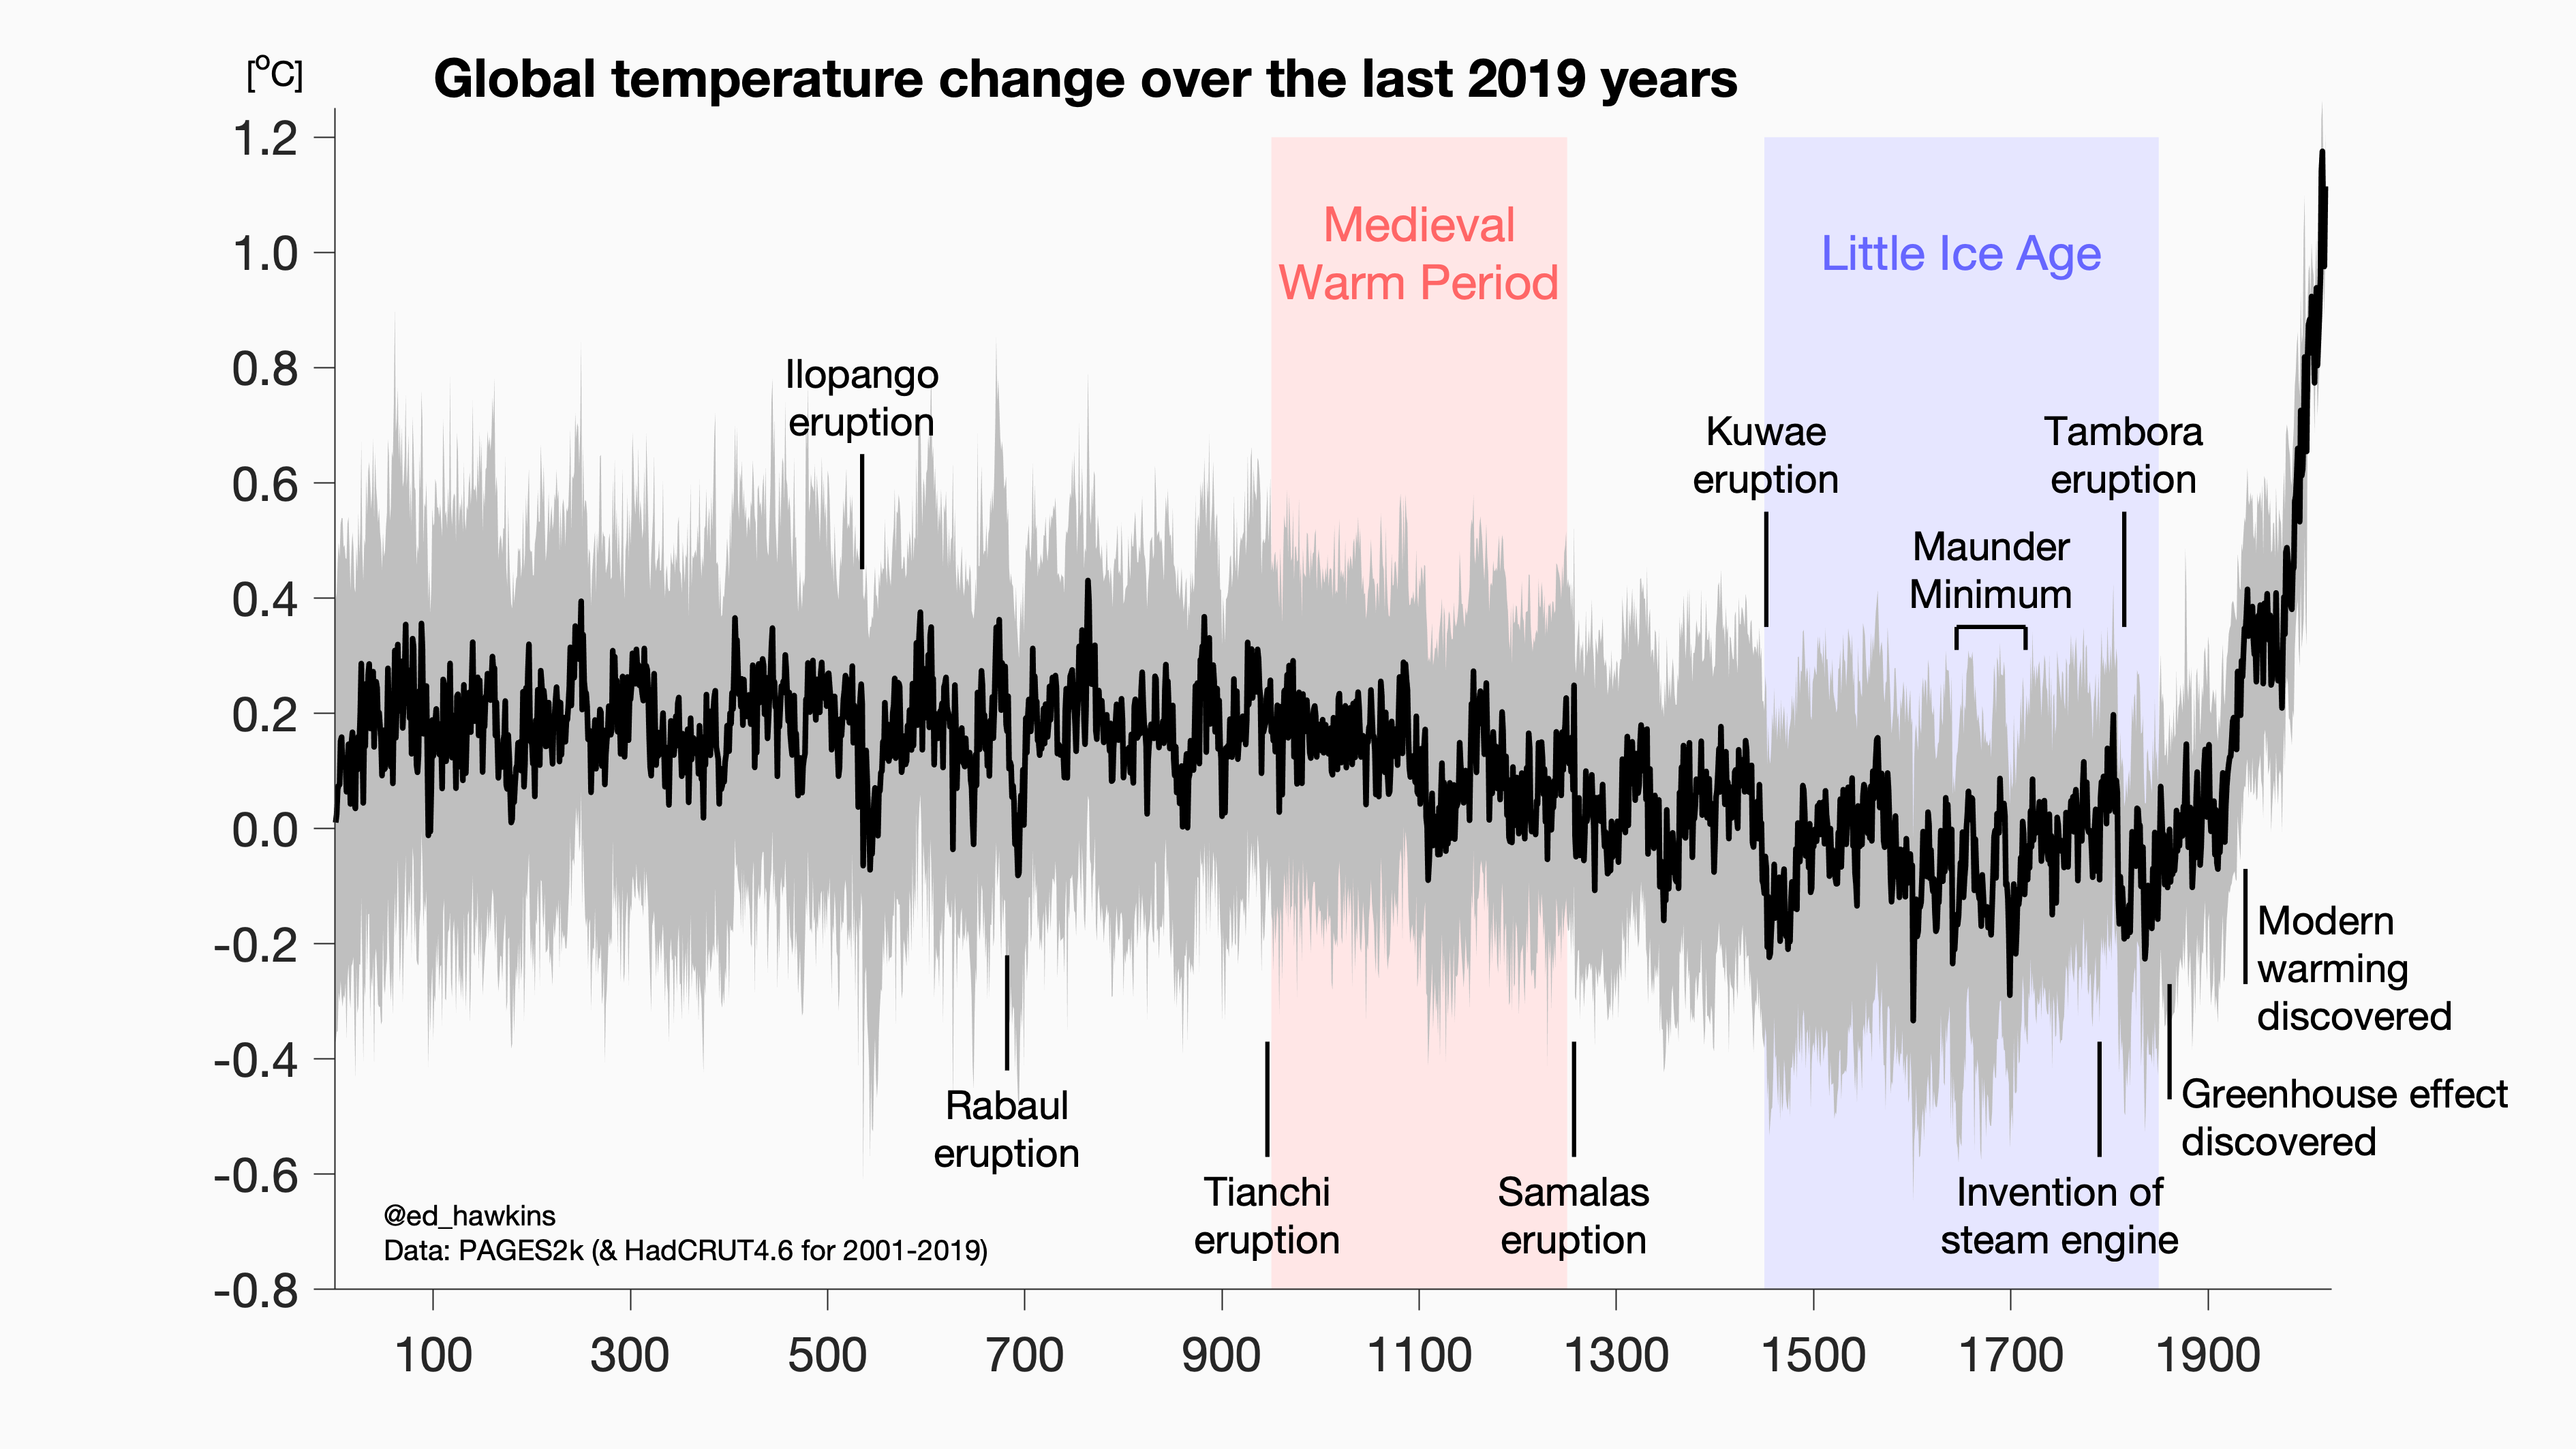
\includegraphics[width=\textwidth]{../grafici/lia_mwp-1.png}
  \caption{Temperature reconstructions by Ed Hawkins using data from PAGES2k showing the Little Ice Age cooling period.}
  \label{fig:lia}
\end{figure}

The Little Ice Age was not, however, a period of uniform cooling. There is a growing consensus in the literature that it was rather a period of local and temporary cooling characterized by increased climate variability and extreme weather events. \textcite{Neukom2019} show that there is no evidence for globally coherent cold epochs during the Common Era; rather, the LIA manifested as a complex mosaic of regional anomalies. Even within Europe, the cooling was asymmetric. Proxy data reveal that while England and the Low Countries experienced winters 0.8--1.2°C colder than the modern average, the Eastern Mediterranean saw a milder anomaly of around 0.5--1.0°C \parencite{Xoplaki2024}. Similarly, summer temperatures in the Central Eastern Alps dropped by up to 1.5°C during the coldest decades \parencite{LarocqueTobler2019}, whereas Southern European summers remained broadly stable. In parts of the Mediterranean, the cooling was modest enough that growing-season conditions were not substantially impaired; some areas even recorded slightly enhanced spring precipitation and warmer early-summer temperatures during the LIA \parencite{Luterbacher2004, Wanner2022}, a contrast that will matter for understanding the asymmetric agricultural responses below.

\textcite{Wanner2022} and \textcite{Luterbacher2004} emphasize that the European LIA was primarily characterized by extreme seasonality: while winter average temperatures were lower, summer conditions were highly variable, oscillating between cold, wet seasons and periods of drought. This spatiotemporal variability meant that the economic impact was geographically uneven. The cooling was particularly pronounced in the North Atlantic and Alpine regions, whereas parts of Eastern Europe and the Mediterranean experienced different hydrological regimes \parencite{Hughes2014, Gaceu2025}. For the agrarian economies of Northern and Central Europe, the climatic shift was profound; for the South, it was comparatively more modest.

\begin{table}[h!]
  \centering
  \begin{tabular}{lrr}
    \toprule
    Region & Summer JJA (°C) & Annual (°C) \\
    \midrule
    Anatolia       & 20.99 & 12.47 \\
    Balkans        & 20.01 & 11.34 \\
    Eastern\_Europe & 16.94 &  7.75 \\
    Iberia         & 19.46 & 13.09 \\
    Italy          & 21.07 & 13.01 \\
    Scandinavia\_S  & 15.09 &  5.67 \\
    UK             & 13.83 &  8.36 \\
    \bottomrule
  \end{tabular}
  \caption{Average temperatures (1000--1990 CE) by region. \emph{Summer JJA}: mean June--August temperature from the Updated EuroMed2k reconstruction \parencite{Ljungqvist2019}. \emph{Annual}: mean annual temperature from the PAGES~2k EU2k2 BHM reconstruction, computed as ensemble-median anomaly plus CRU~TS3.22 1961--1990 baseline.}
  \label{tab:regional_temps}
\end{table}

It is unsurprising, therefore, that the climatic cooling of the seventeenth century often coincided with agrarian and social crises, especially in areas with pre-existing harsh climatic conditions. A famous example comes from the Norse colonies in Greenland: settlements established during the preceding Medieval Warm Period faced increasingly difficult conditions \parencite{dugmore_cultural_2012}. After around 1250, the climate became much colder and stormier, making agriculture marginal. Paleodietary sources indicate that by around 1300, settlers had strongly reduced their consumption of agricultural products, deriving over 75\% of their food from seal hunting and marine resources. By the mid-fourteenth century, trade with Europe had diminished and the Norse colony was in decline; isolated by sea ice and lacking sufficient local resources, the population abandoned the island or perished by the early fifteenth century.
\subsection*{Temperature and agricultural productivity}
To understand why the same climatic event, the Little Ice Age, had heterogeneous effects across regions, we must consider the relationship between temperature and agricultural productivity. This relationship is non-linear and hump-shaped, sometimes described as an ``inverted U-shape'' or asymmetric curve: productivity increases with temperature up to an optimal point, then decreases.
Agronomical research by \textcite{Schlenker2009} shows that agricultural production is strongly dependent on temperature and the length of the growing season, with yields declining sharply when climatic conditions fall outside the optimal range. Specifically, for modern agriculture, they identify critical temperature thresholds beyond which productivity plummets: 29°C for maize, 30°C for soybeans, and 32°C for cotton. While pre-industrial Europe relied on different staples, the underlying physiological principle is consistent: there is a minimum heat accumulation, often measured in Growing Degree Days (GDD), required for a crop to mature.
As \textcite{Burke2015} shows, on a macroeconomic scale, per capita production peaks at around 13°C. This non-linearity implies that the effect of a temperature change on the agricultural sector depends critically on the initial climatic condition. The regional summer temperature averages in \Cref{tab:regional_temps} illustrate this asymmetry starkly: Mediterranean regions (Italy 21°C JJA, Iberia 19°C JJA; annual means 13°C) sit far above this threshold, while the UK (13.8°C JJA; 8.4°C annual) and southern Scandinavia (15.1°C JJA; 5.7°C annual) are already near or at the lower margin of viable cultivation.

Recent work by \textcite{hu2024climate} reinforces this perspective to analyze crop yield responses. Their findings highlight that while extreme heat negatively impacts yields, moderate temperature increases in certain contexts can be beneficial, particularly when interacting with precipitation patterns. As shown in \Cref{fig:hu_response}, the response of crop yields to temperature is non-linear and highly dependent on the baseline climate, supporting the hypothesis that temperature reduction affects mostly regions on the left of the curve, where the temperature is at or below the optimal temperature.

\begin{figure}[h!]
  \centering
  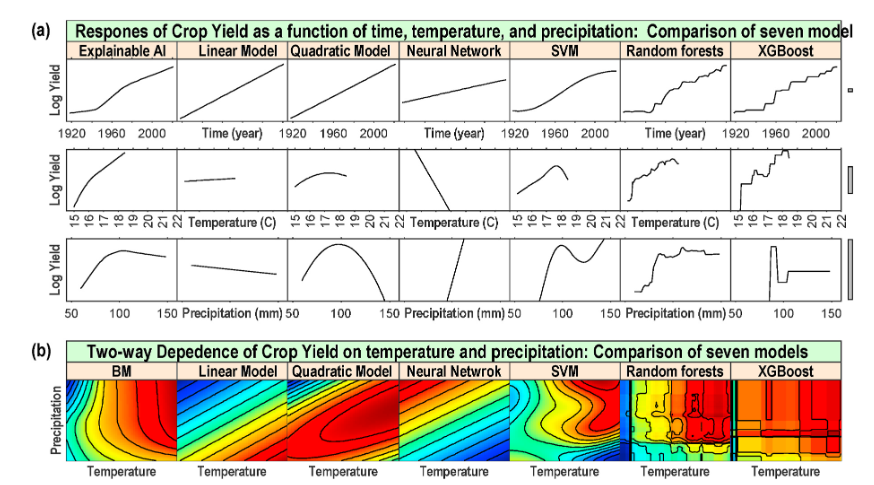
\includegraphics[width=\textwidth]{../grafici/response_to_climate_change.png}
  \caption{Responses of Crop Yield as a function of time, temperature, and precipitation. Source: \textcite{hu2024climate}.}
  \label{fig:hu_response}
\end{figure}

Following this logic, we can divide the European regions into two groups:
\begin{itemize}
  \item \textbf{Regions above the optimum} (e.g., Mediterranean Southern Europe, with mean summer temperatures of 19--21°C; see \Cref{tab:regional_temps}): LIA cooling had paradoxical and ambiguous effects here. Warmer spring temperatures accelerated crop maturation, allowing wheat to complete its growth cycle before the late-summer Mediterranean drought \parencite{OddoErdkamp2025}. At the same time, the LIA increased summer precipitation in parts of the region \parencite{Luterbacher2004, Wanner2022}, further attenuating typical heat-and-drought stress. Both mechanisms buffered agricultural output from the cooling shock.
  \item \textbf{Regions near or below the optimum} (e.g., Northern Atlantic Europe, with UK at 13.8°C JJA / 8.4°C annual and southern Scandinavia at 15.1°C JJA / 5.7°C annual; see \Cref{tab:regional_temps}): These regions were precariously positioned on the lower tail of the productivity curve. Any further cooling reduced GDD below the minimum threshold for reliable cultivation, leading to sharp declines in agricultural product.
\end{itemize}

Climatic data for this period are scarce and lack fine spatial granularity. Nonetheless, two considerations support an asymmetric reading. First, existing proxy reconstructions suggest that the LIA cooling was, if anything, more pronounced in Northern Europe than in the Mediterranean \parencite{Neukom2019, Luterbacher2004}, making a uniform-decline assumption conservative. Second, even under that conservative assumption, the non-linear temperature--productivity relationship documented above implies that Northern regions, already operating near the lower boundary of viable cultivation, would have borne a disproportionate share of the productivity loss. This logic motivates what I call the ``caloric squeeze'' hypothesis: a severe tightening of the margin between agricultural output and subsistence needs (\Cref{fig:kilocalories}).

\subsection*{The caloric squeeze and the subsistence constraint}
Caloric intake has a hard biological floor: prolonged deficits lead to starvation, disease, and death. This constraint fundamentally shapes the response to productivity shocks. In pre-industrial societies, the Little Ice Age cooling imposed a double burden. On one hand, it reduced crop yields; on the other, it increased the biophysical cost of survival. \textcite{MartinezGonzalez2020} note that during the Maunder Minimum, colder temperatures raised the basal metabolic rate (BMR) required for thermoregulation by up to 17--50\%, effectively increasing the subsistence threshold \(\bar{y}\) while simultaneously lowering land productivity.

Consider a simple production function:
\[
  y = f(\text{labor}, \text{land}, \text{climate}).
\]
Land is fixed. When the climate deteriorates, reducing effective productivity and increasing caloric needs, households face a stark choice: either reduce consumption below subsistence and perish, or increase labor input to maintain output and survive. This reaction to exogenous shocks pushes toward induced innovation, where scarcity and crises act as catalysts for change \parencite{Hicks1932, Boserup1965}.

We call this adaptation ``forced industriousness.''
Historical evidence shows that starting in the 16th century, many European countries experienced a significant increase in labor input, typically attributed in part to the Protestant work ethic \parencite{Weber1905}. However, current quantitative literature suggests that the massive increase in labor input observed in pre-industrial England was not a voluntary choice driven by religion, cultural shifts, or consumerism, but a survival-led necessity. \textcite{AllenWeisdorf2011} demonstrate that between 1600 and 1800, rural workers drastically increased their annual working days, often doubling them from 150 to nearly 300, not to acquire luxury goods, but to maintain a stable subsistence level amidst falling real wages and rising food prices. This ``hardship-led industriousness'' \parencite{HumphriesWeisdorf2019} suggests that the compression of the caloric margin was the primary engine forcing households in colder, more vulnerable regions to extract more output from the same land, with labor as the only available margin.

This response requires the climatic pressure to be manageable: too severe a shock, such as in the Greenland case, leads to collapse; too mild, as in the Mediterranean core, reduces the incentive to innovate. We argue that regions like England or the Netherlands faced a pressure strong enough to break the stagnation but not catastrophic enough to cause collapse. That intermediate pressure, significant but survivable, was what produced the industrious response.

\subsection*{Learning-by-doing: from crisis to innovation}

The increase in labor hours had an important side effect: it accelerated the accumulation of productive knowledge.
Following \textcite{Arrow1962}, this is learning-by-doing: technical progress arises from experience accumulated through production. The more hours farmers work, the more they experiment, adapt, and discover new techniques. In the framework I am going to present in the next section, the rate of technological accumulation is directly linked to labor effort: \(A_{t+1} = A_t[1 + \rho h_t^\gamma - \delta_A]\), where \(h_t\) represents hours worked and \(\rho\) the learning rate.
This mechanism implies that the regions forced to work hardest during the Little Ice Age, the colder regions, accumulated technology faster. The harsh climate, by compressing leisure and forcing continuous agricultural effort, inadvertently created a hothouse of innovation. Farmers developed new rotations (including fodder crops like clover and turnips) to sustain livestock through longer winters \parencite{Tello2017}, better drainage systems \parencite{Skoglund2023}, improved fertilization techniques, and more resilient crop varieties. As \textcite{Costello2023} documents, in pastoral regions like Scotland and Ireland, farmers engaged in small-scale cereal cultivation on uplands specifically to buffer against the risk of fodder shortages due to harsher winters. Similar patterns of land-use adaptation and diversification have been documented in southern Sweden, where drainage improvements and the introduction of new crop varieties (such as two-row barley) increased resilience to excess moisture \parencite{Skoglund2023}.
\textcite{Tello2017} argue that the English agricultural revolution was ``more a discovery than an invention, induced by a combination of climate challenges and market incentive''. English farmers reacted to lower temperatures by increasing the flow of organic matter and manure into the soil; when temperatures rose again, the faster mineralization of soil organic matter led to bountiful yields that reinforced these innovative strategies. Colder temperatures and shorter growing seasons also disrupted ecological equilibria: prolonged cooling led to a decline in soil bacterial activity, reducing nitrogen release and diminishing land fertility \parencite{Tello2017}.
Several empirical studies support this dynamic. \textcite{DeDreu2018} show, through an analysis of 500 years of European data, that prolonged cold climate periods coincided with higher rates of scientific and technological innovation, even after controlling for population. Specifically, a 0.5°C drop in mean temperatures is associated with a 0.3--0.6 standard deviation increase in the rate of recorded innovations. The authors find that this link runs through economic pressure: colder temperatures raised grain prices, which in turn incentivized the search for new solutions. It is not that cold ``inspires'' innovation directly, but it generates the scarcity that makes innovation necessary. \textcite{MartinezGonzalez2020}, analyzing England during 1645--1740, find that climate change during the Maunder Minimum negatively affected agricultural yields but also accelerated structural change in the agrarian sector, potentially contributing to the onset of the English Agricultural Revolution and the broader European divergence.
The induced innovation hypothesis from climate shocks finds a parallel in 
prehistory. \textcite{Matranga2024} demonstrates that increased climatic 
seasonality---greater contrast between seasons, with long periods of 
scarcity---drove the Neolithic revolution and the adoption of sedentary 
agriculture among hunter-gatherer populations. The same logic applies to 
pre-industrial Europe: where climatic stress was most acute, the incentive
to innovate was strongest, and where it was absent, so was the urgency
to change.
The warmer South exemplifies this contrapositive. Mediterranean farmers, operating closer to the climatic optimum, had less urgency to intensify their labor or experiment with new techniques.
\subsection*{Heterogeneous responses: trade, adaptation, and social crises}
Different societies responded to the Little Ice Age in different ways, depending on institutional and geographic conditions.
Interregional grain trade grew substantially during the cold period, as grain moved from surplus to deficit regions. \textcite{Waldinger2022} provides econometric evidence that trading cities were able to offset the negative effects of the cooling, whereas isolated regions suffered significantly more. This suggests that market integration and commercial networks cushioned the worst effects of climatic stress.

Moreover, the Southern European agricultural model exhibited structural resilience. \textcite{OddoErdkamp2025} show that in Tuscany, the Little Ice Age manifested through harsh winters and increased hydrological instability, particularly in fragile landscapes like the \textit{Crete Senesi} where excessive rainfall caused significant soil erosion. However, within this generally cooler regime, ``warmer'' springs and summers were actually beneficial for wheat maturation. By accelerating the growth cycle, higher temperatures allowed the grain to be harvested in early summer, effectively ``escaping'' the peak drought of July and August \parencite{OddoErdkamp2025}. Institutions like the \textit{Annona}, the public grain administration, acted as shock absorbers, stabilizing supply and prices during harvest failures. Unlike the North, where cold meant yield failure, the South capitalized on a diversified agricultural portfolio. The cultivation of olives, vines, and legumes alongside cereals acted as natural insurance: specific climatic conditions detrimental to wheat might spare or even favor other crops. This biodiversity, combined with established market networks and institutional buffers, reduced the volatility of the food supply in the Mediterranean relative to the precarious monocultures of the North.

These differential outcomes are, in aggregate, the early signature of what historians call the Little Divergence. Northern economies that faced the sharpest climatic pressure responded with the most rapid adaptation. The Dutch Republic prospered during the coldest decades of the Little Ice Age \parencite{Pfister2022}; \textcite{Allen2003} classifies the Dutch and English economies as high-wage exceptions precisely in this period. \textcite{Degroot2018} documents how Dutch merchants exploited harvest failures elsewhere and inventors adapted to the cold: iceboats for frozen canals, improved windmills. English farmers increased their labor input substantially and pioneered new agricultural rotations \parencite{AllenWeisdorf2011}. In Scandinavia, drainage improvements and new crop varieties were adopted in direct response to harsher growing conditions \parencite{Skoglund2023}. The pattern is consistent: where climatic pressure was greatest, adaptation came earliest.

Conversely, in regions where these buffers failed, the stress of agricultural failure has been linked to darker social phenomena. \textcite{Iyigun2017} document a strong quantitative correlation between long-term cooling trends and the frequency of conflict in Europe and Asia. The erosion of the agricultural surplus weakened state capacity and intensified competition for shrinking resources, feeding a cycle of instability. \textcite{Behringer1999} similarly connects intense witch-hunting episodes to the desperation caused by climate-induced agricultural failures. As \textcite{Zhang2011} documents, the coldest periods were associated with significant declines in agricultural production and bio-productivity, precipitating a sequence of social crises---including wars, famines, epidemics, and migration---which contributed to a population collapse around 1650.
\subsection*{From crisis to surplus: post-LIA innovations and demographic-industrial growth}
A related question is whether the innovations developed during the Little Ice Age had lasting effects: whether the techniques and institutional changes adopted out of necessity also generated a productive surplus once the climate improved. The thesis is that they did: adaptations born of crisis laid the groundwork for the agricultural and demographic expansion of the 18th and 19th centuries.
Historical evidence supports this reading. With the gradual improvement in climate during the 18th century, regions that had innovated early could capitalize on new techniques: more efficient rotations, organic fertilization (through nitrogen-fixing legumes like clover), improved drainage and irrigation systems, and the spread of high-yield imported crops raised agricultural output beyond pre-crisis levels. \textcite{Tello2017} argue that investments in soil fertility made to survive the cold---such as intensive manuring and legume rotations---created a ``delayed reward'': when temperatures rose, the faster mineralization of the accumulated organic matter led to bountiful yields that reinforced these innovative strategies. This agricultural surplus had far-reaching consequences.

First, it supported rapid demographic growth: increased per capita caloric availability reduced famine incidence and increased fertility and survival, leading European population to unprecedented growth between 1750 and 1850. Quantitative estimates indicate that a single innovation---the widespread introduction of the potato---was responsible for a significant share of this growth. According to \textcite{NunnQian2011}, the adoption of the potato imported from the Americas accounts for a substantial share of Old World population growth and urbanization in the 18th and 19th centuries. In Scandinavia, \textcite{Skoglund2023} confirms that the introduction of the potato and new rotations allowed agricultural production to outpace demographic growth, definitively breaking the Malthusian constraints that had previously limited expansion.

A second consequence of the agricultural surplus was the activation of proto-industrial growth. With more food available at relatively lower prices, an increasing share of the population could turn to non-agricultural activities: emigration to cities supported early industrialization, while rural areas developed small-scale manufactures such as domestic textile work. This was a two-way relationship. Agricultural surplus enabled urban growth, but growing urban demand also pulled agricultural production forward. Following a Thünen logic, \textcite{KopsidisWolf2012} and \textcite{Pfister2022} show that proximity to urban markets pushed farmers toward more intensive techniques, reinforcing the interdependence between city and countryside. The agricultural surplus ensured that this transition occurred without the Malthusian bottleneck: in short, north-western Europe entered the 19th century with a larger, better-nourished population more free to engage in emerging sectors.
\subsection*{North--South divergence: the role of climate in European asymmetry}
Together, these elements point toward a climate-based explanation of intra-European divergence. The North--South divergence thesis postulates that countries in northern and Atlantic Europe, experiencing a more severe impact from the Little Ice Age, were forced to adapt earlier and more radically, developing agricultural innovations and modern institutions already in the pre-industrial era; conversely, southern (Mediterranean) and more temperate regions felt less the bite of cold climate and therefore delayed abandoning traditional systems.
Comparative historical data support this reading. In countries like Sweden or England, the agricultural sector in the late 18th century was already growing faster than population, signaling continuous productivity gains \parencite{OlssonSvensson2010}. By contrast, Mediterranean countries like Italy remained in a stagnant condition until well into the 19th century, with agricultural output per worker even lower than in the medieval era \parencite{FedericoMalanima2004}. This ``little divergence'' within Europe, preceding the 19th-century Great Divergence on a global scale, can partly be explained by geo-climatic differences: cold zones had to face marginal harvests and greater risks (late frosts, short summers, etc.), while warm zones like Southern Europe experienced more stable conditions that reduced the urgency of change.
For example, England and the Netherlands, characterized by cool oceanic climates and strong seasonal oscillations, precociously adopted reforms such as enclosures and four-field rotation, and improved agricultural markets and property rights to incentivize productive investments. Such measures, as noted by \textcite{OlssonSvensson2010}, were decisive in enabling farmers to increase production and react to shocks; they also reveal the greater institutional flexibility of Northern Europe relative to the South. In the South, by contrast, traditional agrarian models (such as extensive cereal latifundia, widespread use of fallow, scarce varietal innovation) persisted longer, partly because the climatic pressure that, in our framework, acts as the primary trigger of agrarian change was comparatively absent. A milder and more stable climate reduced the cost of maintaining traditional systems.
\subsection*{Reassessing the Protestant work ethic}
The thesis advanced in this work has important implications for one of the most influential explanations of the Great Divergence: Max Weber's hypothesis that the Protestant Reformation, with its emphasis on hard work and worldly success as signs of divine favor, was a primary driver of Northern European economic development.
Weber's argument has been highly influential, and the correlation between Protestantism and early industrialization is undeniable. However, our framework suggests a different interpretation: the greater labor effort observed in Protestant Northern Europe may not have been primarily caused by religious ideology, but rather by climatic necessity.
The Reformation spread most successfully in Northern Europe, precisely the regions most severely affected by the Little Ice Age during the seventeenth century (England, the Netherlands, Scandinavia). This geographic overlap is unlikely to be coincidental. It can be argued that the observed ``work ethic'' of these regions was, at its core, a rational response to environmental pressure rather than a cultural or theological innovation. Farmers in England, the Netherlands, and Scandinavia worked longer hours because they had to; their survival depended on it.

An important example is provided by the removal of holy days following the Reformation. \textcite{AllenWeisdorf2011} document that in 1536, England abolished 49 saints' days on which work had been forbidden. Weber might interpret this as evidence of Protestant asceticism; our framework suggests a different reading. The removal of these days coincided with a period when rural workers needed to increase their annual working days simply to maintain subsistence consumption in the face of falling real wages and rising food prices. The Reformation thus provided the \textit{theological justification} (abolition of the cult of saints) for what was already an \textit{economic necessity} (working more days to avoid starvation).

This interpretation does not imply that the Reformation was irrelevant. Religious and cultural factors likely served as catalysts and reinforcers of the industrious behavior that climate had already made necessary. Protestant theology may have legitimized hard work, making it socially acceptable and morally virtuous. However, the fundamental impetus, the first-order reason why these populations worked more in the first place, may have been environmental and not ideological.


\begin{figure}[h!]
  \centering
  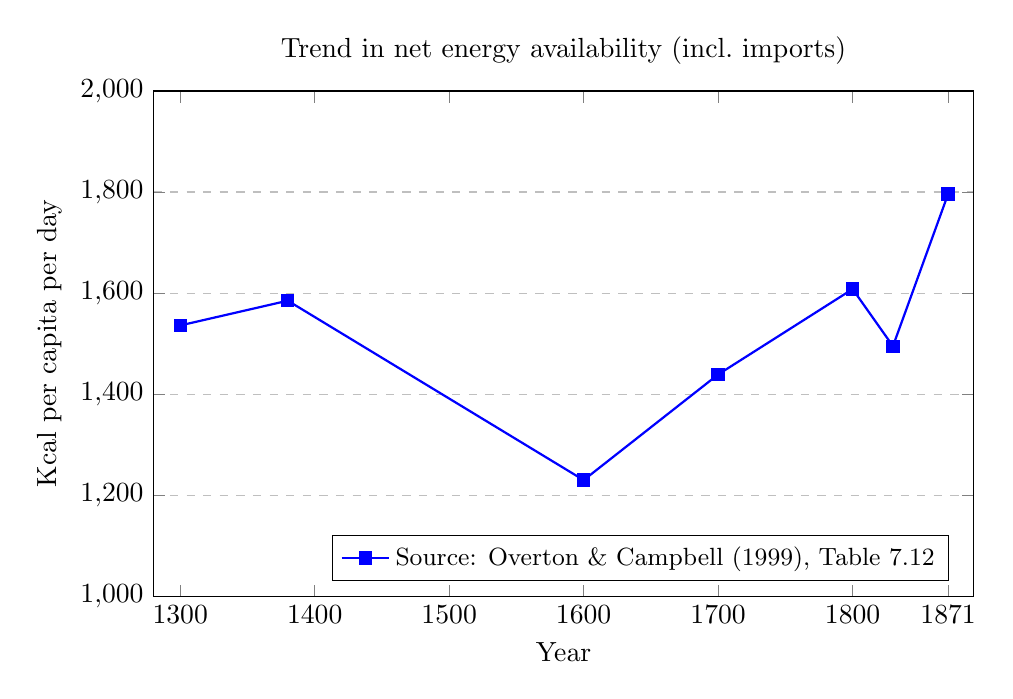
\begin{tikzpicture}
    \begin{axis}[
        width=12cm,
        height=8cm,
        title={Trend in net energy availability (incl.\ imports)},
        xlabel={Year},
        ylabel={Kcal per capita per day},
        xmin=1280, xmax=1890,
        ymin=1000, ymax=2000,
        xtick={1300, 1400, 1500, 1600, 1700, 1800, 1871},
        xticklabel style={/pgf/number format/1000 sep=},
        ymajorgrids=true,
        grid style=dashed,
        legend pos=south east,
        legend style={font=\small}
      ]

      % Data from Table 7.12 (Net b - Including imports)
      % For 1300 and 1380 we use the midpoint of the reported intervals.
      \addplot[
        color=blue,
        mark=square*,
        thick
      ]
      coordinates {
        (1300, 1536)  % Midpoint of 1446--1626
        (1380, 1585)  % Midpoint of 1500--1669
        (1600, 1230)
        (1700, 1439)
        (1800, 1608)
        (1830, 1495)
        (1871, 1796)
      };

      % Legend with source
      \addlegendentry{Source: Overton \& Campbell (1999), Table 7.12}

    \end{axis}
  \end{tikzpicture}
  \caption{Estimated per-capita kilocalories available (grain and potatoes) in England, 1300--1871. Data include imports and are net of seed, losses, and feed.}
  \label{fig:kilocalories}
\end{figure}

\subsection*{Plan of the paper}
I develop the arguments just explained, formally and empirically. \Cref{sec:induced_innovation} presents a model of Malthusian dynamics with induced innovation driven by climate shocks. The model formalizes the intuition that adverse climatic conditions, by forcing households to work harder to maintain subsistence, generate technological accumulation through learning-by-doing. I derive comparative statics showing how labor supply responds to climatic pressure and demonstrate conditions under which regions facing greater stress accumulate technology faster.
\Cref{sec:long_run} extends the analysis to long-run dynamics, showing how the technological lead accumulated during the Little Ice Age translates into an earlier escape from the Malthusian trap and an earlier demographic transition. I demonstrate that the same climatic shock that caused short-run hardship becomes the engine of long-run divergence.
The model is calibrated to match pre-industrial European conditions, and numerical simulations are presented in Section 5. I compare two stylized regions, a ``Cold'' North and a ``Warm'' South, subject to the same physical temperature shock but experiencing asymmetric productivity impacts due to their different positions on the temperature-productivity curve. The simulations reproduce the key features of the Little Divergence: the North's earlier agricultural take-off, its accumulation of technological advantage, and the eventual reversal of fortune.
Before the formal model, I review empirical evidence on the LIA's agricultural effects and the induced innovation literature.

\section{Model}

\subsection*{Environment and timing}

Time is discrete, \(t=0,1,2,\dots\). A representative agrarian economy is described by three state variables:
\[
  X_t \equiv (A_t, L_t, T_t),
\]
where
\begin{itemize}
  \item \(A_t>0\) is a stock of production-enhancing knowledge or technology;
  \item \(L_t>0\) is population size;
  \item \(T_t>0\) represents an exogenous climatic shifter (e.g., mean temperature or length of the growing season). For parsimony, \(T_t\) is interpreted as the \textit{effective} climate term in production and can absorb both yield effects and climate-driven shifts in subsistence needs (e.g., thermoregulatory costs).
\end{itemize}

Land \(R>0\) is fixed and uniformly distributed across the population. Within each period \(t\) the sequence of events is:
\begin{enumerate}
  \item State \((A_t,L_t,T_t)\) is given.
  \item Households choose labor \(h_t\in[0,1]\) (hours as a share of time endowment); leisure is \(\ell_t=1-h_t\).
  \item Output and consumption per capita \(c_t\) are realized from production.
  \item Births and deaths occur; \(A_{t+1}\) and \(L_{t+1}\) are determined; the climate shifter \(T_{t+1}\) is realised.
\end{enumerate}

\subsection*{Technology and production}

Production is organized at the household level with a simple Malthusian technology. Effective labor per capita is given by \(h_t\), and land enters via a congestion term. We assume
\begin{equation}
  \begin{split}
    c_t &\;=\; y_t \\
    &\;=\; A_t\,T_t\,\kappa(L_t)\,f(h_t),
  \end{split}
  \label{eq:prod_def}
\end{equation}
where
\[
  \kappa(L_t) \equiv \left(\frac{R}{L_t}\right)^{1-\alpha},
  \qquad
  \alpha\in(0,1),
\]
and \(f:[0,1]\to\mathbb{R}_+\) is a reduced-form productivity of hours satisfying only:
\begin{equation}
  f(0)=0,\quad f'(h)>0,\quad f''(h)\le 0\quad\text{for all }h\in(0,1].
  \label{eq:F_assumptions}
\end{equation}
The term \(\kappa(L_t)\) captures Malthusian congestion due to land scarcity, with \(1-\alpha\) governing its strength. We abstract from physical capital accumulation, focusing instead on knowledge capital \(A_t\).

For some results we will use the benchmark functional form
\begin{equation}
  f(h) = h^\eta,\qquad \eta\in(0,1),
  \label{eq:f_power}
\end{equation}
where \(\eta\) governs the diminishing returns to labor hours. The term \(\kappa(L_t) = (R/L_t)^{1-\alpha}\) captures Malthusian congestion. Per-capita output scales with population as \(c_t \propto L_t^{-(1-\alpha)}\); higher \(\alpha\) implies weaker congestion.

\textit{Assumption (Atomistic Households).} Each household is atomistic and does not internalize the effect of its labor choice on aggregate knowledge accumulation \(A_{t+1}\) (which depends on aggregate labor input \(H_t \equiv h_t L_t\)). Thus, the optimization problem is static.

\subsection*{Preferences and the subsistence constraint}

Households value consumption and leisure. We impose a strict subsistence requirement \(\bar y>0\):
\begin{equation}
  U(c_t,\ell_t) = u(c_t) + v(\ell_t), \qquad \ell_t=1-h_t,
  \label{eq:U_def}
\end{equation}
subject to the feasibility constraint:
\begin{equation}
  c_t \ge \bar y \quad \text{if feasible}.
  \label{eq:subsistence_constraint}
\end{equation}
Formally, if the maximum possible production \(y_{max} = A_t T_t \kappa(L_t) f(1)\) is less than \(\bar y\), the household works \(h_t=1\) to minimize the caloric deficit (Famine regime). If \(y_{max} \ge \bar y\), the household maximizes utility subject to \(c_t \ge \bar y\).

Standard properties apply: \(u'(c)>0, u''(c)<0\) and \(v'(\ell)>0, v''(\ell)<0\).

\subsection*{The static problem within a period}

Given \((A_t,L_t,T_t)\), let \(\Pi_t \equiv A_t T_t \kappa(L_t)\) denote total factor productivity. The household solves:
\begin{equation}
  \max_{h_t\in[0,1]} \; u(\Pi_t f(h_t)) + v(1-h_t)
  \quad\text{subject to}\quad
  \Pi_t f(h_t) \ge \bar{y} \; (\text{if } \Pi_t f(1) \ge \bar{y}).
  \label{eq:static_problem}
\end{equation}

Define the minimal labor required to meet subsistence (if feasible):
\begin{equation}
  h_t^{\text{need}}(A_t,L_t,T_t)
  \;=\;
  f^{-1}\!\Bigg(\frac{\bar y}{A_t T_t \kappa(L_t)}\Bigg).
  \label{eq:h_need_closed}
\end{equation}

\textit{Assumption (Survival Rule).} If \(\Pi_t f(1) < \bar y\) (subsistence infeasible), households supply \(h_t=1\) to maximize caloric intake.

\begin{lemma}[Optimal Labor Choice]
  \label{lem:corner}
  The optimal labor choice \(h_t^*\) is characterized by two regimes based on productivity \(\Pi_t\):

  \begin{enumerate}
    \item \textbf{Infeasible Regime (Famine):} If \(\Pi_t f(1) < \bar y\), by the Survival Rule:
      \[ h_t^* = 1. \]

    \item \textbf{Feasible Regime:} If \(\Pi_t f(1) \ge \bar y\), the household chooses \(h_t^* \in [h_t^{\text{need}}, 1]\). The solution is:
      \[ h_t^* = \max \left\{ h_t^{\text{need}}, h_t^{unc} \right\}, \]
      where \(h_t^{unc}\) is the solution to the unconstrained first-order condition:
      \[ u'(\Pi_t f(h)) \Pi_t f'(h) = v'(1-h). \]
  \end{enumerate}
\end{lemma}

\begin{proof}
  Part (i) follows directly from the Survival Rule.
  Part (ii): The constraint \(c \ge \bar y\) binds \(h \ge h^{\text{need}}\). The objective function is strictly concave on this domain. If the unconstrained peak \(h^{unc}\) falls below \(h^{\text{need}}\), the constraint binds (\(h^* = h^{\text{need}}\)). If \(h^{unc} \ge h^{\text{need}}\), the interior solution is optimal.
\end{proof}

\begin{corollary}[Corner vs.\ Interior Solution]
  \label{cor:corner}
  In the feasible regime:
  \begin{enumerate}
    \item \textbf{Subsistence Trap:} Households are stuck at \(c_t = \bar{y}\) (\(h_t^* = h_t^{\text{need}}\)) when productivity is low enough that the income effect of leisure dominates:
      \[ u'(\bar y) \cdot \Pi_t f'(h^{\text{need}}) \le v'(1 - h^{\text{need}}). \]
    \item \textbf{Interior Growth:} Households choose \(c_t > \bar{y}\) (\(h_t^* > h^{\text{need}}\)) when productivity is sufficiently high.
  \end{enumerate}
\end{corollary}

\begin{remark}[The Greenland Paradox]
  \label{rem:greenland}
  One caveat: our model predicts innovation only if the shock is survivable (\(\Pi_t f(1) \ge \bar{y}\)). If climatic conditions deteriorate to the point where even maximum effort cannot sustain the population, as was the case for the Norse settlements in Greenland during the LIA, the result is collapse, not induced innovation. The ``industrious response'' is conditional on the feasibility of the subsistence constraint.
\end{remark}

\subsection*{Demographic Dynamics: A Reduced-Form Approach}
\label{sec:demography}

To close the model, we specify the dynamics of population \(L_t\). The demographic block is deliberately kept in reduced form. Our goal is to import the main qualitative insights of \textcite{GalorWeil2000} without adding a full quality--quantity optimization layer that would complicate the model without altering its central mechanism. The three Galor--Weil dynamics we wish to preserve are: (i) a positive Malthusian link between income and fertility; (ii) an endogenous brake on fertility as technology accumulates, through the quality--quantity trade-off; and (iii) a demographic transition once productivity crosses a critical threshold. We implement all three through simple functional forms on birth and death rates. Population evolves as:
\begin{equation}
  L_{t+1} \;=\; L_t\,\exp(n_t - d_t),
  \label{eq:L_law}
\end{equation}
where \(n_t\) is the birth rate and \(d_t\) is the death rate. This exponential formulation ensures \(L_t > 0\) for all \(t\).

The mortality rate \(d_t\) depends negatively on the subsistence ratio \(x_t \equiv c_t/\bar y\):
\begin{equation}
  d(x_t) = \mu \, x_t^{\epsilon_d},
\end{equation}
with \(\mu > 0\) and \(\epsilon_d < 0\).

The fertility rate \(n_t\) is governed by a reduced-form function:
\begin{equation}
  n(x_t, A_t) \;=\; \bar{n} \cdot x_t^{\epsilon_n} \cdot \frac{1}{1 + \omega A_t}.
  \label{eq:fertility_def}
\end{equation}\footnote{Following \textcite{GalorWeil2000}, we assume that technological progress raises the return to human capital, thereby increasing the opportunity cost of raising children (the quality-quantity trade-off). This effect operates even at the subsistence level, reflecting the increased time cost of child-rearing in a more complex technological environment.}

\section{Induced Innovation via Labor-Leisure Choice}
\label{sec:induced_innovation}

\subsection*{The results of induced industriousness}

Building on the labor choice problem, we derive how effort responds to the three state variables: climatic pressure (\(T_t\)), technology (\(A_t\)), and population (\(L_t\)).

\begin{prop}[Climate, technology and Malthusian congestion]
  \label{prop:CS}
  In the feasible region where the subsistence constraint binds (i.e.\ \(c^* = \bar y\)), the optimal labor choice \(h_t^*\) is given by:
  \begin{equation}
    h_t^* = f^{-1}\!\Bigg(\frac{\bar y}{A_t T_t \kappa(L_t)}\Bigg).
    \label{eq:h_star_closed}
  \end{equation}
  It follows that \(h_t^*\) is strictly decreasing in \(A_t\) and \(T_t\), and strictly increasing in \(L_t\):
  \[
    \frac{\partial h_t^*}{\partial A_t} < 0,
    \qquad
    \frac{\partial h_t^*}{\partial T_t} < 0,
    \qquad
    \frac{\partial h_t^*}{\partial L_t} > 0.
  \]
\end{prop}

\begin{proof}
  By \eqref{eq:F_assumptions}, \(f\) is strictly increasing and hence \(f^{-1}\) is strictly increasing. The term \(\bar y/(A_t T_t \kappa(L_t))\) is strictly decreasing in \(A_t\) and \(T_t\), and strictly increasing in \(L_t\) (because \(\kappa(L_t)\) falls in \(L_t\)). Monotonicity of \(f^{-1}\) delivers the sign results.
\end{proof}

Proposition~\ref{prop:CS} provides the core economic intuition of our model. In a subsistence economy, households work as little as possible to secure \(\bar y\). Consequently, any exogenous stressor, be it a cooling climate (\(T_t \downarrow\)) or a larger population (\(L_t \uparrow\)), forces households to increase their labor input \(h_t\) to survive.

\begin{remark}[The Little Ice Age vs. The Black Death]
  \label{rem:LIA_vs_BD}
  It is instructive to contrast the Little Ice Age with a demographic shock like the Black Death. The Black Death was a sudden labor supply shock that increased the land-to-labor ratio (\(R/L \uparrow\)), thereby raising per-capita productivity and allowing more leisure. In contrast, the Little Ice Age was a productivity shock (\(T \downarrow\)). Although the LIA also led to a population decline due to starvation, the climatic deterioration was the primary driver of the crisis. Households were forced to work harder (\(h \uparrow\)) because the drop in \(T\) outweighed the marginal benefit of reduced congestion from lower \(L\). 
\end{remark}

\subsection*{Learning-by-doing and the innovation feedback}

Knowledge accumulation is linked to the time spent in production. We assume the following law of motion for \(A_t\):
\begin{equation}
  A_{t+1} = A_t \big[1 + \rho\, H_t^\gamma - \delta_A \big],
  \qquad \rho>0,\ \gamma\in(0,1],\ \delta_A \ge 0.
  \label{eq:A_law}
\end{equation}
The term \(\rho H_t^\gamma\) represents the learning-by-doing rate, explicitly grounding technical change in the accumulation of experience through labor conceptualized by \textcite{Arrow1962}. This specification allows for a mild scale effect in learning: a larger population generates more aggregate experience, but with diminishing returns governed by \(\gamma\). \(\delta_A\) represents knowledge depreciation.

To ensure the model captures the historical reality of pre-industrial stagnation, we impose that in the absence of climatic shocks (normal times), the knowledge generated by subsistence labor roughly balances depreciation:
\begin{equation}
  \rho (H_{subsistence})^\gamma \approx \delta_A.
  \label{eq:stagnation_condition}
\end{equation}
Here \(H_{subsistence}\) denotes aggregate labor input in the subsistence steady state.
This condition formally defines the ``trap'': without the exogenous stimulus of the Little Ice Age, the net growth of technology is negligible (\(\Delta A_t \approx 0\)), and the economy remains indefinitely in the Malthusian steady state.

Through \eqref{eq:A_law}, the industrious response to climate shocks has a permanent effect on the technological trajectory.

\begin{prop}[The Escape Mechanism]
  \label{prop:escape}
  Assume the functional forms \(u(c) = \frac{c^{1-\sigma}}{1-\sigma}\), \(v(\ell) = \psi \frac{(1-h)^{1-\nu}}{1-\nu}\) and \(f(h)=h^\eta\). In the \textbf{Interior Regime} (\(c^* > \bar{y}\)), assume the parameter conditions \(\eta(1-\sigma) < 1\) and \(\nu > 0\). If the income effect is sufficiently weak relative to the substitution effect (governed by the curvature parameter \(0 < \sigma < 1\)), then optimal hours \(h_t^*\) are strictly increasing in total factor productivity \(\Pi_t\) (and thus in \(A_t\)):
  \[ \frac{\partial h_t^*}{\partial \Pi_t} > 0. \]
\end{prop}

\begin{proof}
  In the interior regime, the first-order condition is \(u'(c)\Pi f'(h) - v'(1-h) = 0\). Substituting the functional forms:
  \[ \eta \Pi^{1-\sigma} h^{\eta(1-\sigma)-1} - \psi (1-h)^{-\nu} = 0. \]
  Define the LHS function \(G(h, \Pi) \equiv \eta \Pi^{1-\sigma} h^{\eta(1-\sigma)-1} - \psi (1-h)^{-\nu}\).
  By the Implicit Function Theorem, \(\frac{\partial h^*}{\partial \Pi} = - \frac{\partial G / \partial \Pi}{\partial G / \partial h}\).
  First, differentiate with respect to \(\Pi\):
  \[ \frac{\partial G}{\partial \Pi} = \eta (1-\sigma) \Pi^{-\sigma} h^{\eta(1-\sigma)-1}. \]
  Since \(\sigma < 1\), this term is strictly positive (\(\frac{\partial G}{\partial \Pi} > 0\)).
  Second, differentiate with respect to \(h\):
  \[ \frac{\partial G}{\partial h} = \eta \Pi^{1-\sigma} [\eta(1-\sigma)-1] h^{\eta(1-\sigma)-2} - \psi \nu (1-h)^{-\nu-1}. \]
  The second term (\(-\psi \nu (1-h)^{-\nu-1}\)) is strictly negative since \(\nu>0\). The first term is negative if \(\eta(1-\sigma) < 1\). Given our assumption (and since \(\eta < 1\) and \(\sigma < 1\)), both terms are negative, so \(\frac{\partial G}{\partial h} < 0\).
  Thus, \(\frac{\partial h^*}{\partial \Pi} = - \frac{(+)}{(-)} > 0\).
\end{proof}

\begin{remark}[Industriousness and the Substitution Effect]
  \label{rem:sigma}
  Proposition~\ref{prop:escape} provides the formal underpinning of what \textcite{Voth2001} and \textcite{DeVries2008} call the ``Industrious Revolution.'' Once productivity is high enough to push the economy into the interior regime, a low curvature \(\sigma < 1\) in \(u(c)\) ensures that the substitution effect dominates the income effect, sustaining high labor input as \(A\) grows. This dynamic allows the technological lead accumulated under climatic stress to persist and compound after the climate recovers. The specific value of \(\sigma\) is discussed in the calibration (Section~\ref{sec:calibration}).
\end{remark}

\subsection*{The Mechanism of the Trap and the Escape}

The results above describe a specific dynamic in pre-industrial growth, which we call the ``Leisure Trap.''

In our framework, as long as households are bound by the subsistence requirement, technological improvements (\(A_t \uparrow\)) do not automatically translate into higher consumption. Instead, they allow households to meet their subsistence needs with fewer hours of work. Since agents value leisure, they respond to ``good times'' by reducing labor effort. Crucially, because technological progress is driven by learning-by-doing, this reduction in labor effort acts as a brake on innovation. Thus, in a benign environment, the economy tends to settle into a low-work, low-growth equilibrium: prosperity limits the very accumulation of knowledge needed to sustain it.

This mechanism implies that autonomous improvements are insufficient to trigger a transition. The system requires a shock strong enough to break the preference for leisure.

The Little Ice Age provides exactly this shock. The climatic deterioration (\(T_t \downarrow\)) acts as a negative productivity shock. In the short run, households must work significantly harder (\(h_t \uparrow\)) just to maintain subsistence consumption. However, this ``forced industriousness'' has a dynamic benefit. The surge in labor effort accelerates the creation of knowledge via learning-by-doing, forcing the economy to accumulate technology at a rate that would not be chosen voluntarily in a stable climate.

If the shock persists, the stock of technology \(A_t\) accumulates to a critical level. Once productivity is sufficiently high, the incentive structure flips: the economy crosses into the ``Interior Solution'' regime where higher productivity makes consumption more attractive relative to leisure. This sets off a self-reinforcing process of rising hours, rising consumption, and sustained technological growth that eventually breaks the Malthusian trap.

This escape requires a ``critical mass'' of accumulated knowledge. If the Little Ice Age were to end prematurely, before \(A_t\) has reached the takeoff threshold, the incentive to innovate would vanish. Without the pressure of the cold climate, households would revert to their preference for leisure, causing labor hours \(h\) to drop. If \(h\) falls below the level required to offset knowledge depreciation (\(\delta_A\)), the economy would gradually slide back into stagnation. European geographical divergence can thus be read as a product of the LIA's varying duration and intensity: only where climatic stress lasted long enough did a structural shift occur and the agricultural revolution take root permanently.

\subsection*{Testable Hypotheses}
The model generates three qualitative predictions. Each finds support in the empirical literature reviewed above; the simulations in Section~5 show that the calibrated model reproduces them quantitatively.

\begin{enumerate}
  \item \textbf{Timing of Divergence:} Regions experiencing more severe or persistent cooling during the Little Ice Age should exhibit earlier signs of agricultural productivity growth compared to milder regions. This is consistent with the historical record for Northern Europe relative to the Mediterranean \parencite{OlssonSvensson2010, MartinezGonzalez2020}.
  \item \textbf{Intensity of Shocks:} There should be a positive correlation between the magnitude of the climatic shock and the subsequent rate of innovation, provided the shock does not exceed the survival threshold. \textcite{DeDreu2018} provide direct econometric evidence for this relationship across five centuries of European data.
  \item \textbf{Reversal of Fortune:} Areas that were marginally less productive in the short run due to climatic stress should eventually overtake climatically stable regions in the long run through accumulated induced innovation, the early signature of the Little Divergence documented by \textcite{Pfister2022} and \textcite{Allen2003}.
\end{enumerate}

\section{Long-Run Dynamics and the Great Divergence}
\label{sec:long_run}

\subsection*{The Takeoff Threshold}

Combined with the demographic laws in \Cref{sec:demography}, the accelerated growth of \(A\) in regions hit by the LIA leads to an earlier demographic transition.

\begin{prop}[Existence of a Transition Threshold]
  \label{prop:transition}
  Consider the fertility function \(n(x, A)\) given in \eqref{eq:fertility_def}.
  \begin{enumerate}
    \item \textbf{Subsistence Regime:} If the economy is constrained at subsistence (\(c_t = \bar{y}\)), fertility \(n_t\) is strictly decreasing in technology \(A_t\).
    \item \textbf{Interior Regime:} In the interior solution regime (\(c_t > \bar{y}\)), there exists a critical technological level \(A^*\) such that the relationship between fertility and technology is hump-shaped: \(n_t\) increases with \(A_t\) for \(A_t < A^*\) (if the income effect dominates) and decreases for \(A_t > A^*\).
  \end{enumerate}
\end{prop}

\begin{proof}
  We analyze the partial equilibrium response of fertility \(n_t\) to an increase in technology \(A_t\), holding \(L_t\) constant (and thus \(\kappa(L_t)\) constant).

  \paragraph{Case 1: Subsistence Regime.}
  Consider the regime defined in Lemma~\ref{lem:corner} where optimal consumption is corner-constrained: \(c_t^\star = \bar{y}\). In this case, the relative income \(x_t \equiv c_t^\star/\bar{y} = 1\) is constant and independent of \(A_t\). Substituting this into the fertility function \eqref{eq:fertility_def}:
  \[
    n_t|_{c=\bar{y}} \;=\; \bar{n} \cdot (1)^{\epsilon_n} \cdot \frac{1}{1 + \omega A_t} \;=\; \frac{\bar{n}}{1 + \omega A_t}.
  \]
  Differentiating with respect to \(A_t\):
  \[
    \frac{\partial n_t}{\partial A_t} \;=\; -\frac{\omega \bar{n}}{(1 + \omega A_t)^2} \;<\; 0.
  \]
  Thus, in the strict subsistence regime, technological improvements lead solely to a decline in fertility (due to the pure substitution/complexity effect).

  \paragraph{Case 2: Interior Solution Regime.}
  Consider the regime where technology is sufficiently high such that households choose an interior solution \(c_t^\star > \bar{y}\). Recall from Lemma \ref{lem:corner} that in the interior regime \(h_t^*\) satisfies \(u'(c_t^\star)\Pi_t f'(h_t^*)=v'(1-h_t^*)\), which implies optimal consumption \(c_t^\star(A_t)\) is strictly increasing in \(A_t\). Let \(x_t(A_t) = c_t^\star(A_t)/\bar{y}\).
  Taking the natural logarithm of \eqref{eq:fertility_def}:
  \[
    \ln n_t = \ln \bar{n} + \epsilon_n \ln x_t(A_t) - \ln(1 + \omega A_t).
  \]
  Differentiating with respect to \(A_t\):
  \[
    \frac{\partial \ln n_t}{\partial A_t} \;=\; \epsilon_n \frac{1}{x_t} \frac{\partial x_t}{\partial c_t} \frac{\partial c_t}{\partial A_t} - \frac{\omega}{1 + \omega A_t}
    \;=\; \epsilon_n \frac{1}{c_t} \frac{\partial c_t}{\partial A_t} - \frac{\omega}{1 + \omega A_t}.
  \]
  Let \(\varepsilon_{c,A} \equiv \frac{\partial \ln c_t}{\partial \ln A_t} > 0\) denote the elasticity of consumption to technology. We can rewrite the derivative as:
  \[
    \frac{\partial \ln n_t}{\partial A_t} \;=\; \frac{1}{A_t} \left[ \epsilon_n \, \varepsilon_{c,A} \;-\; \frac{\omega A_t}{1 + \omega A_t} \right].
  \]
  Fertility increases if and only if the breakdown of the Malthusian trap (income effect) dominates the complexity cost:
  \[
    \epsilon_n \, \varepsilon_{c,A} \;>\; \frac{\omega A}{1 + \omega A}.
  \]
  For low levels of \(A\) (but high enough to be in the interior regime), the term \(\frac{\omega A}{1+\omega A}\) is small, allowing the income effect to dominate (\(\partial n / \partial A > 0\)). As \(A \to \infty\), the term \(\frac{\omega A}{1+\omega A} \to 1\). A necessary condition for the demographic transition is that the income elasticity of births is not too high. Specifically, as technological progress makes consumption more efficient (\(\varepsilon_{c,A} \to 1\)), we require \(\epsilon_n < 1\) for the fertility rate to eventually decline. This condition is consistent with empirical evidence for pre-industrial economies, which typically exhibits birth-income elasticities significantly below unity \parencite{Clark2008}.
  The threshold \(A^*\) is defined as the point in the interior regime where this inequality flips.
\end{proof}

This threshold defines the escape from the Malthusian trap. In our climate experiment, the colder region (North) is forced into higher \(h\) and thus higher accumulation of \(A\). If the shock is sufficiently persistent, \(A_{North}\) crosses \(A^*\) while \(A_{South}\) remains trapped in stagnation.

\section{Simulation Results}
This section presents numerical simulations of the model calibrated for the period 1000--1900 AD. We compare two regions: a ``Warm'' region (South) and a ``Cold'' region (North). We posit that region-specific agricultural productivity \(T_{r,t}\) is a non-linear function of physical temperature \(\mathcal{T}_{r,t}\):
\begin{equation}
  T_{r,t} = g(\mathcal{T}_{r,t}).
\end{equation}
We interpret \(g(\cdot)\) as globally hump-shaped in temperature, but we work on the \textit{cold margin} (the left tail), where \(g'(\cdot)>0\) and the response to cooling is steep and non-linear. Thus, while both regions experience the same physical cooling \(\Delta \mathcal{T}\) during the Little Ice Age (approx.\ 1275--1850), the \textit{effective} productivity shock is asymmetric:
\begin{itemize}
  \item \textbf{North (Cold Margin):} \(T_{\text{North},t}\) drops significantly (\(T_{shock} \approx 10\%\)) due to the non-linear response of crop yields to shorter growing seasons.
  \item \textbf{South (Warm Core):} The same cooling has a negligible effect on \(T_{\text{South},t}\) as the region remains well within the optimal growing envelope.
\end{itemize}
To keep the experiment transparent while matching the historical timing, we implement climate forcing as a reduced-form multiplicative wedge on productivity. For the North, \(T_{\text{North},t}\) declines linearly from 1 to \(1-T_{shock}\) between 1275 and 1645, remains at \(1-T_{shock}\) during the Maunder Minimum (1645--1715), and then recovers linearly to 1 by 1850. For the South, we set \(T_{\text{South},t}=1\) throughout. This yields a ``similar climatic event'' that generates divergent economic incentives due to different initial geographic conditions.

\subsection*{Parameter Calibration}
\label{sec:calibration}

The model is calibrated to represent the technological and demographic conditions of Europe over 1000--1900 AD. \Cref{tab:parameters} summarizes all parameter values together with their empirical source or calibration target. The calibration strategy follows standard practice in quantitative macroeconomic history \parencite{Lagerlof2006, GalorWeil2000}: a small number of parameters are grounded directly in the empirical literature, while the remaining ones are set to match well-documented historical moments. Each internally calibrated parameter is pinned down by a single target, and no parameter is freely adjusted to improve the fit of the simulations.

\begin{table}[h!]
  \centering
  \caption{Parameter calibration (values used in the simulations)}
  \label{tab:parameters}
  \resizebox{\textwidth}{!}{%
    \begin{tabular}{@{}llrl@{}}
      \toprule
      Parameter & Description & Value & Source / target \\
      \midrule
      \multicolumn{4}{l}{\textit{Empirically grounded}} \\
      \(\alpha\) & Land share (congestion) & 0.50 & \textcite{Allen2000, Crafts1985, VoigtlanderVoth2006} \\
      \(T_{shock}\) & LIA productivity shock (North) & 0.10 & Derived from \textcite{Luterbacher2004, Mann2009} \\
      \(\epsilon_n\) & Birth elasticity & 0.50 & \textcite{WrigleySchofield1981}; see text \\
      \(\epsilon_d\) & Death elasticity & \(-0.40\) & \textcite{Galloway1988}; see text \\
      \midrule
      \multicolumn{4}{l}{\textit{Internally calibrated (moment-matching)}} \\
      \(\sigma\) & CRRA coefficient & 0.30 & Match rising \(h\) 1750--1800 (\textcite{Voth2001}); \(\sigma<1.25\) (\textcite{Chetty2006}) \\
      \(\psi\) & Leisure weight & 0.20 & Match \(h \approx 0.76\) (\textcite{Voth2001}) \\
      \(\rho\) & Learning rate & 0.0021 & Pre-LIA stagnation (Eq.~\ref{eq:stagnation_condition}) \\
      \(\delta_A\) & Knowledge depreciation & 0.0025 & Stagnation: \(\rho H^\gamma \approx \delta_A\) in pre-LIA steady state \\
      \(\gamma\) & Learning curvature & 0.50 & Bounded \(A\) growth without explosive takeoff \\
      \(\bar{n}\) & Baseline birth rate & 0.0215 & Near-zero population growth in pre-LIA steady state \\
      \(\mu\) & Baseline death rate & 0.0155 & Near-zero population growth in pre-LIA steady state \\
      \(\omega\) & Q--Q trade-off & 0.25 & Match demographic transition timing (late 19th c.; \textcite{CoaleWatkins1986}) \\
      \midrule
      \multicolumn{4}{l}{\textit{Normalization and functional forms}} \\
      \(\bar{y}\) & Subsistence requirement & 0.90 & Normalization \\
      \(\eta\) & Labor elasticity in \(f(h)=h^\eta\) & 0.70 & Standard concavity \\
      \(\nu\) & Leisure curvature & 1.00 & Log-leisure benchmark \\
      \(A_0\) & Initial technology & 1.50 & Normalization \\
      \bottomrule
    \end{tabular}%
  }
\end{table}

\subsubsection*{Empirically Grounded Parameters}

\paragraph{Land Share (\(\alpha = 0.50\))}
In pre-industrial agriculture, land was the binding factor of production. \textcite{Allen2000} estimates factor shares for early modern England using probate records and national accounts, finding that land's share in total factor payments ranged between 40\% and 55\%. \textcite{Crafts1985} provides similar estimates for the pre-industrial period. \textcite{VoigtlanderVoth2006} employ \(\alpha = 0.40\) in their Unified Growth model of the British Industrial Revolution. Our choice of \(\alpha = 0.50\) lies within this empirically grounded range and is a standard benchmark in Malthusian models.

\paragraph{Climatic Forcing (\(T_{shock} = 0.10\))}
During the Maunder Minimum (1645--1715), paleoclimatic reconstructions suggest unusually cold European winters; for Europe as a whole, winter average temperatures during 1500--1900 were about 0.5\(^\circ\)C lower than the 20th-century average \parencite{Luterbacher2004, Mann2009}. \textcite{Schlenker2009} document that, in modern agriculture, a 1\(^\circ\)C drop in summer temperature reduces yields by approximately 5\%. Studies of medieval English agriculture find that increased summer rainfall (often associated with cooler conditions) reduces yields by approximately 10\% per standard deviation. \textcite{Parker2013} and \textcite{Campbell2016} document widespread harvest failures and agrarian crises during the coldest phases of the LIA, consistent with yield reductions in the 10--15\% range. We implement the Little Ice Age as a peak 10\% reduction in effective agricultural productivity for the North (\(T_{shock} = 0.10\)). The South is assumed to be unaffected (\(T_{\text{South},t}=1\)).

\paragraph{Demographic Elasticities (\(\epsilon_n = 0.50\), \(\epsilon_d = -0.40\))}
The birth elasticity \(\epsilon_n\) captures the responsiveness of fertility to changes in real income, the core of Malthus's ``preventive check.'' In pre-industrial England, this operated primarily through the age of first marriage: higher wages allowed earlier marriage and thus higher fertility. \textcite{WrigleySchofield1981} document that roughly half of pre-industrial fertility variation was driven by marriage timing, which was itself wage-elastic. Our value of \(\epsilon_n = 0.50\) is consistent with this evidence.

The death elasticity \(\epsilon_d\) captures the ``positive check'', the inverse relationship between income and mortality. When real wages fall, mortality rises due to malnutrition, disease susceptibility, and famine. \textcite{Galloway1988} provides one of the most systematic cross-country estimates of the elasticity of mortality to grain prices in pre-industrial Europe, finding absolute values in the range 0.2--0.5 depending on time period and region (e.g., a cumulative elasticity of 0.38 for non-infant mortality in England during 1675--1755). Galloway estimates the elasticity with respect to grain prices, which serve as a direct inverse proxy for real income in pre-industrial economies where food dominated the consumer price index. Our value of \(|\epsilon_d| = 0.40\) falls within this range.

\subsubsection*{Internally Calibrated Parameters}

Internally calibrated parameters are set to match well-documented historical moments, as described below.

\paragraph{CRRA Coefficient (\(\sigma = 0.30\))}
The parameter \(\sigma\) governs the curvature of the utility function and determines the balance between income and substitution effects. For the ``Industrious Revolution'' documented by \textcite{Voth2001} and \textcite{DeVries2008} to occur, wherein households increase labor supply as productivity rises, the substitution effect must dominate. \textcite{Voth2001} documents that annual working hours in England rose from approximately 2,500 hours in 1750 to approximately 3,300--3,500 hours by 1800, before declining to around 2,700 hours by 1870. The value \(\sigma = 0.30\) is chosen to replicate this positive correlation between technology and labor input during the take-off period. \textcite{Chetty2006} shows that an upward-sloping labor supply curve requires \(\sigma < 1.25\), with most labor supply studies implying values in the range 0.15--1.78 (mean \(\approx 0.71\)). Our value lies within this range and satisfies the theoretical bound.

\paragraph{Leisure Preference (\(\psi = 0.20\))}
The leisure preference parameter \(\psi\) is calibrated to match the approximately 2,500 annual hours observed in mid-18th century England \parencite{Voth2001}. In the simulations, one period is one year and \(h_t\) is mapped to annual hours by normalizing the time endowment to 3,300 hours, so that 2,500 hours corresponds to \(h \approx 0.76\). This is a standard approach in macroeconomic models: \(\psi\) is chosen to match the observed allocation of time between work and leisure.

\paragraph{Learning and Stagnation (\(\rho = 0.0021\), \(\delta_A = 0.0025\), \(\gamma = 0.50\))}
The pre-industrial era was characterized by extremely slow productivity growth. \textcite{CraftsHarley1992} estimate annual TFP growth at approximately \(0.1\%\) for 1760--1800. \textcite{AntrasVoth2003} confirm this using an independent dual method based on factor prices, estimating TFP growth at 0.1--0.2\% per year for 1770--1860. We calibrate \((\rho,\delta_A,\gamma)\) jointly so that, in the pre-LIA steady state, the net growth term in \eqref{eq:A_law} is close to zero (the stagnation condition \eqref{eq:stagnation_condition}): \(\rho H^\gamma \approx \delta_A\). The curvature \(\gamma = 0.50\) ensures diminishing returns to learning-by-doing and prevents explosive knowledge takeoff. Given that learning depends on aggregate labor input \(H_t=h_t L_t\), the parameter \(\rho\) should be interpreted as the productivity of aggregate experience rather than a per-capita learning rate.

\paragraph{Baseline Vital Rates (\(\bar{n} = 0.0215\), \(\mu = 0.0155\))}
The baseline vital rates are chosen to generate near-stationary population dynamics in the pre-LIA steady state, once the income-dependent checks (\(\epsilon_n\), \(\epsilon_d\)) and the technology-dependent quality--quantity term (\(\omega A_t\)) are taken into account in \eqref{eq:fertility_def}. For comparison, \textcite{WrigleySchofield1981} report substantially higher crude vital rates for England; in our reduced-form formulation, \(\bar{n}\) and \(\mu\) should be interpreted as \textit{effective} per-period rates rather than literal crude birth/death rates.

\paragraph{Quality--Quantity Trade-off (\(\omega = 0.25\))}
The parameter \(\omega\) scales the impact of technological progress on the opportunity cost of children, following the theoretical framework of \textcite{GalorWeil2000}. In our model, higher \(\omega\) implies that technological advances more strongly incentivize parents to substitute child ``quality'' (human capital) for ``quantity.'' We calibrate \(\omega\) so that the demographic transition, the sustained decline in fertility, is triggered in the mid-to-late 19th century, consistent with the timing documented by \textcite{CoaleWatkins1986} for Western Europe, where the Total Fertility Rate fell below 4 children per woman between 1870 and 1900.

\subsubsection*{Normalization and Functional Forms}

The subsistence constraint is normalized to \(\bar{y}=0.90\); all output and consumption variables are expressed relative to this threshold. The labor elasticity \(\eta = 0.70\) governs diminishing returns to hours at the intensive margin (\(f(h) = h^\eta\)) and is a conventional functional form assumption. The leisure curvature \(\nu = 1.00\) adopts the log-leisure benchmark. Initial technology \(A_0 = 1.50\) normalizes the starting point of the simulations.

\subsection*{Main Results: From Stagnation to the Little Divergence}

The calibrated model is simulated over the period 1000--1900 AD for two stylized regions: a ``Cold'' North (subject to a 10\% productivity shock during the LIA) and a ``Warm'' South (negligible shock). The results illustrate the full chain of the proposed mechanism: climatic stress \(\to\) forced industriousness \(\to\) accelerated learning \(\to\) technological divergence \(\to\) escape from the Malthusian trap.

\subsubsection*{Labor supply response}

\Cref{fig:sim_hours} displays the labor supply response. In the pre-LIA steady state, both regions exhibit similar hours worked (\(h \approx 0.76\)), consistent with a subsistence-bound equilibrium. As climatic conditions deteriorate after 1275, the North is forced to increase \(h_t\) sharply to maintain output above subsistence, precisely the ``forced industriousness'' predicted by Proposition~\ref{prop:CS}. At the peak of the Maunder Minimum (1645--1715), Northern households work approximately 10\% more hours than their Southern counterparts. Even after the climate recovers, the North maintains higher labor supply: the accumulated technology has pushed the economy into the interior regime where, by Proposition~\ref{prop:escape}, rising productivity sustains high labor input through the substitution effect.

\begin{figure}[h!]
  \centering
  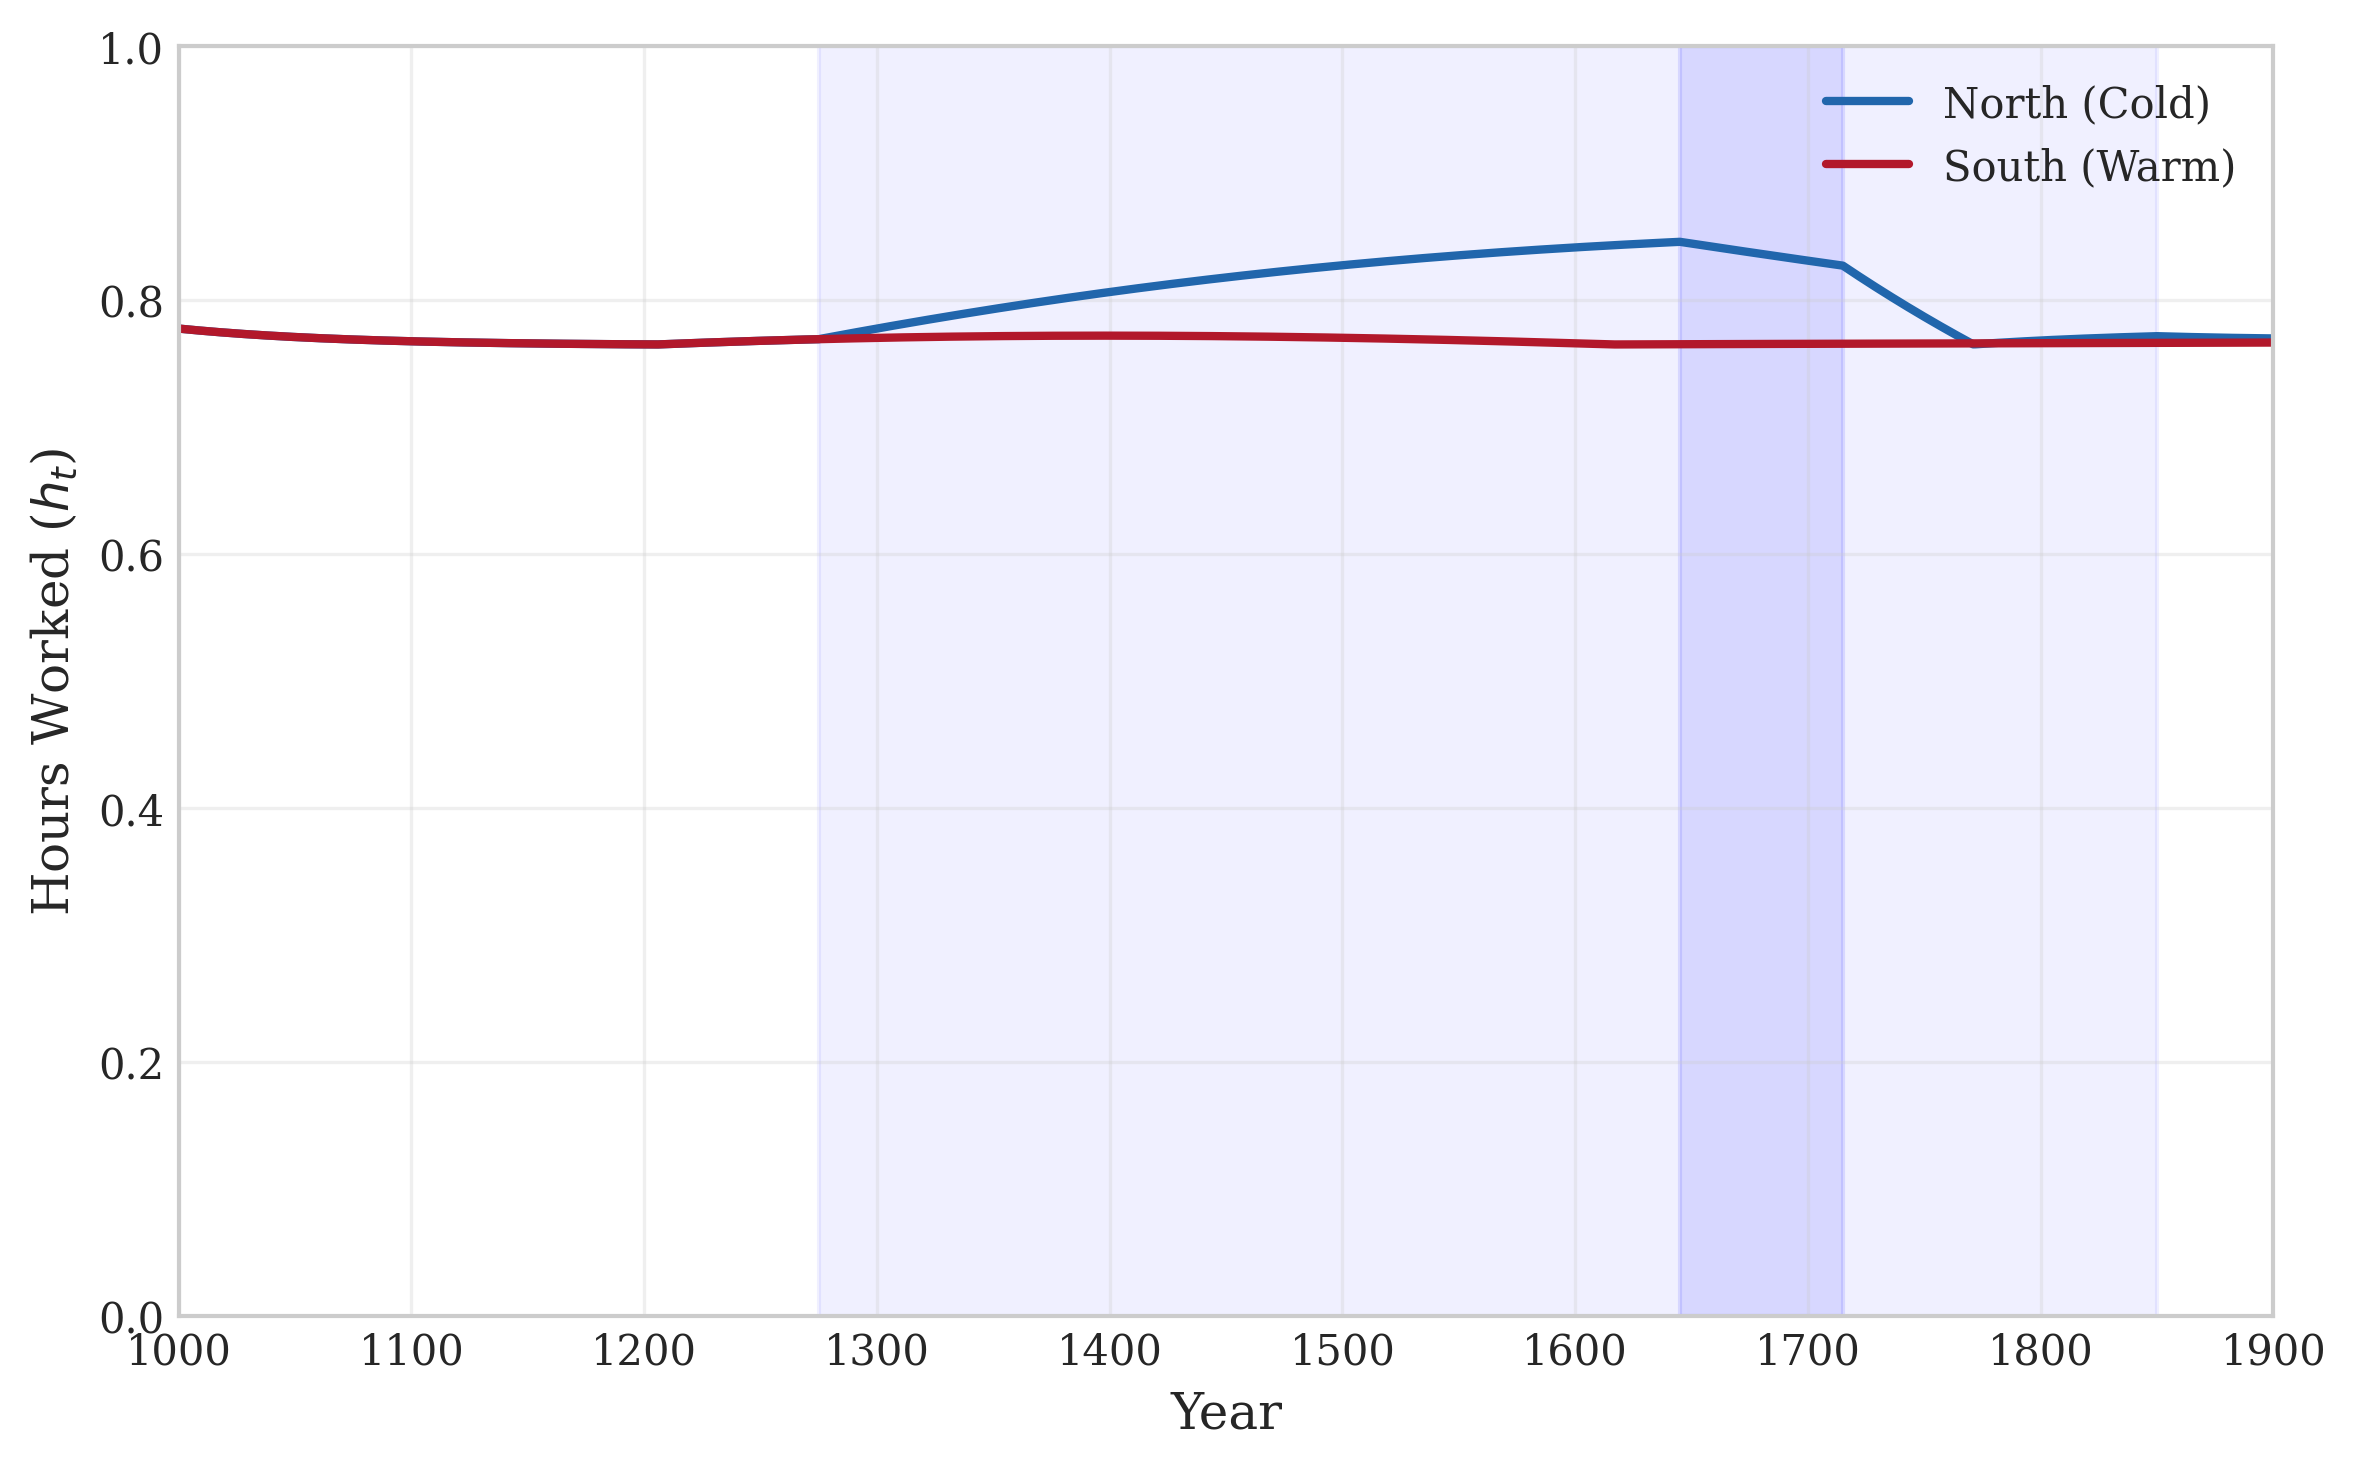
\includegraphics[width=0.9\textwidth]{../grafici_galor/gw_comparison_hours.png}
  \caption{\textbf{Labor Supply.} The climatic shock forces Northern households to increase hours worked (\(h_t\)) to maintain subsistence. After recovery, the substitution effect sustains high labor input in the North. The shaded area marks the Little Ice Age (1275--1850), with the darker band indicating the Maunder Minimum (1645--1715).}
  \label{fig:sim_hours}
\end{figure}

\subsubsection*{Technological divergence}

\Cref{fig:sim_technology} shows the resulting technological trajectories. Both regions start at \(A_0 = 1.5\) and initially follow nearly identical paths. As the LIA intensifies, the higher labor input in the North accelerates learning-by-doing (Eq.~\ref{eq:A_law}), causing the Northern technology stock to grow faster. By 1715 the North has accumulated a measurable lead (\(A_N/A_S \approx 1.03\)), and the gap remains persistent through the post-LIA period (by 1900, \(A_N/A_S \approx 1.03\)).

\begin{figure}[h!]
  \centering
  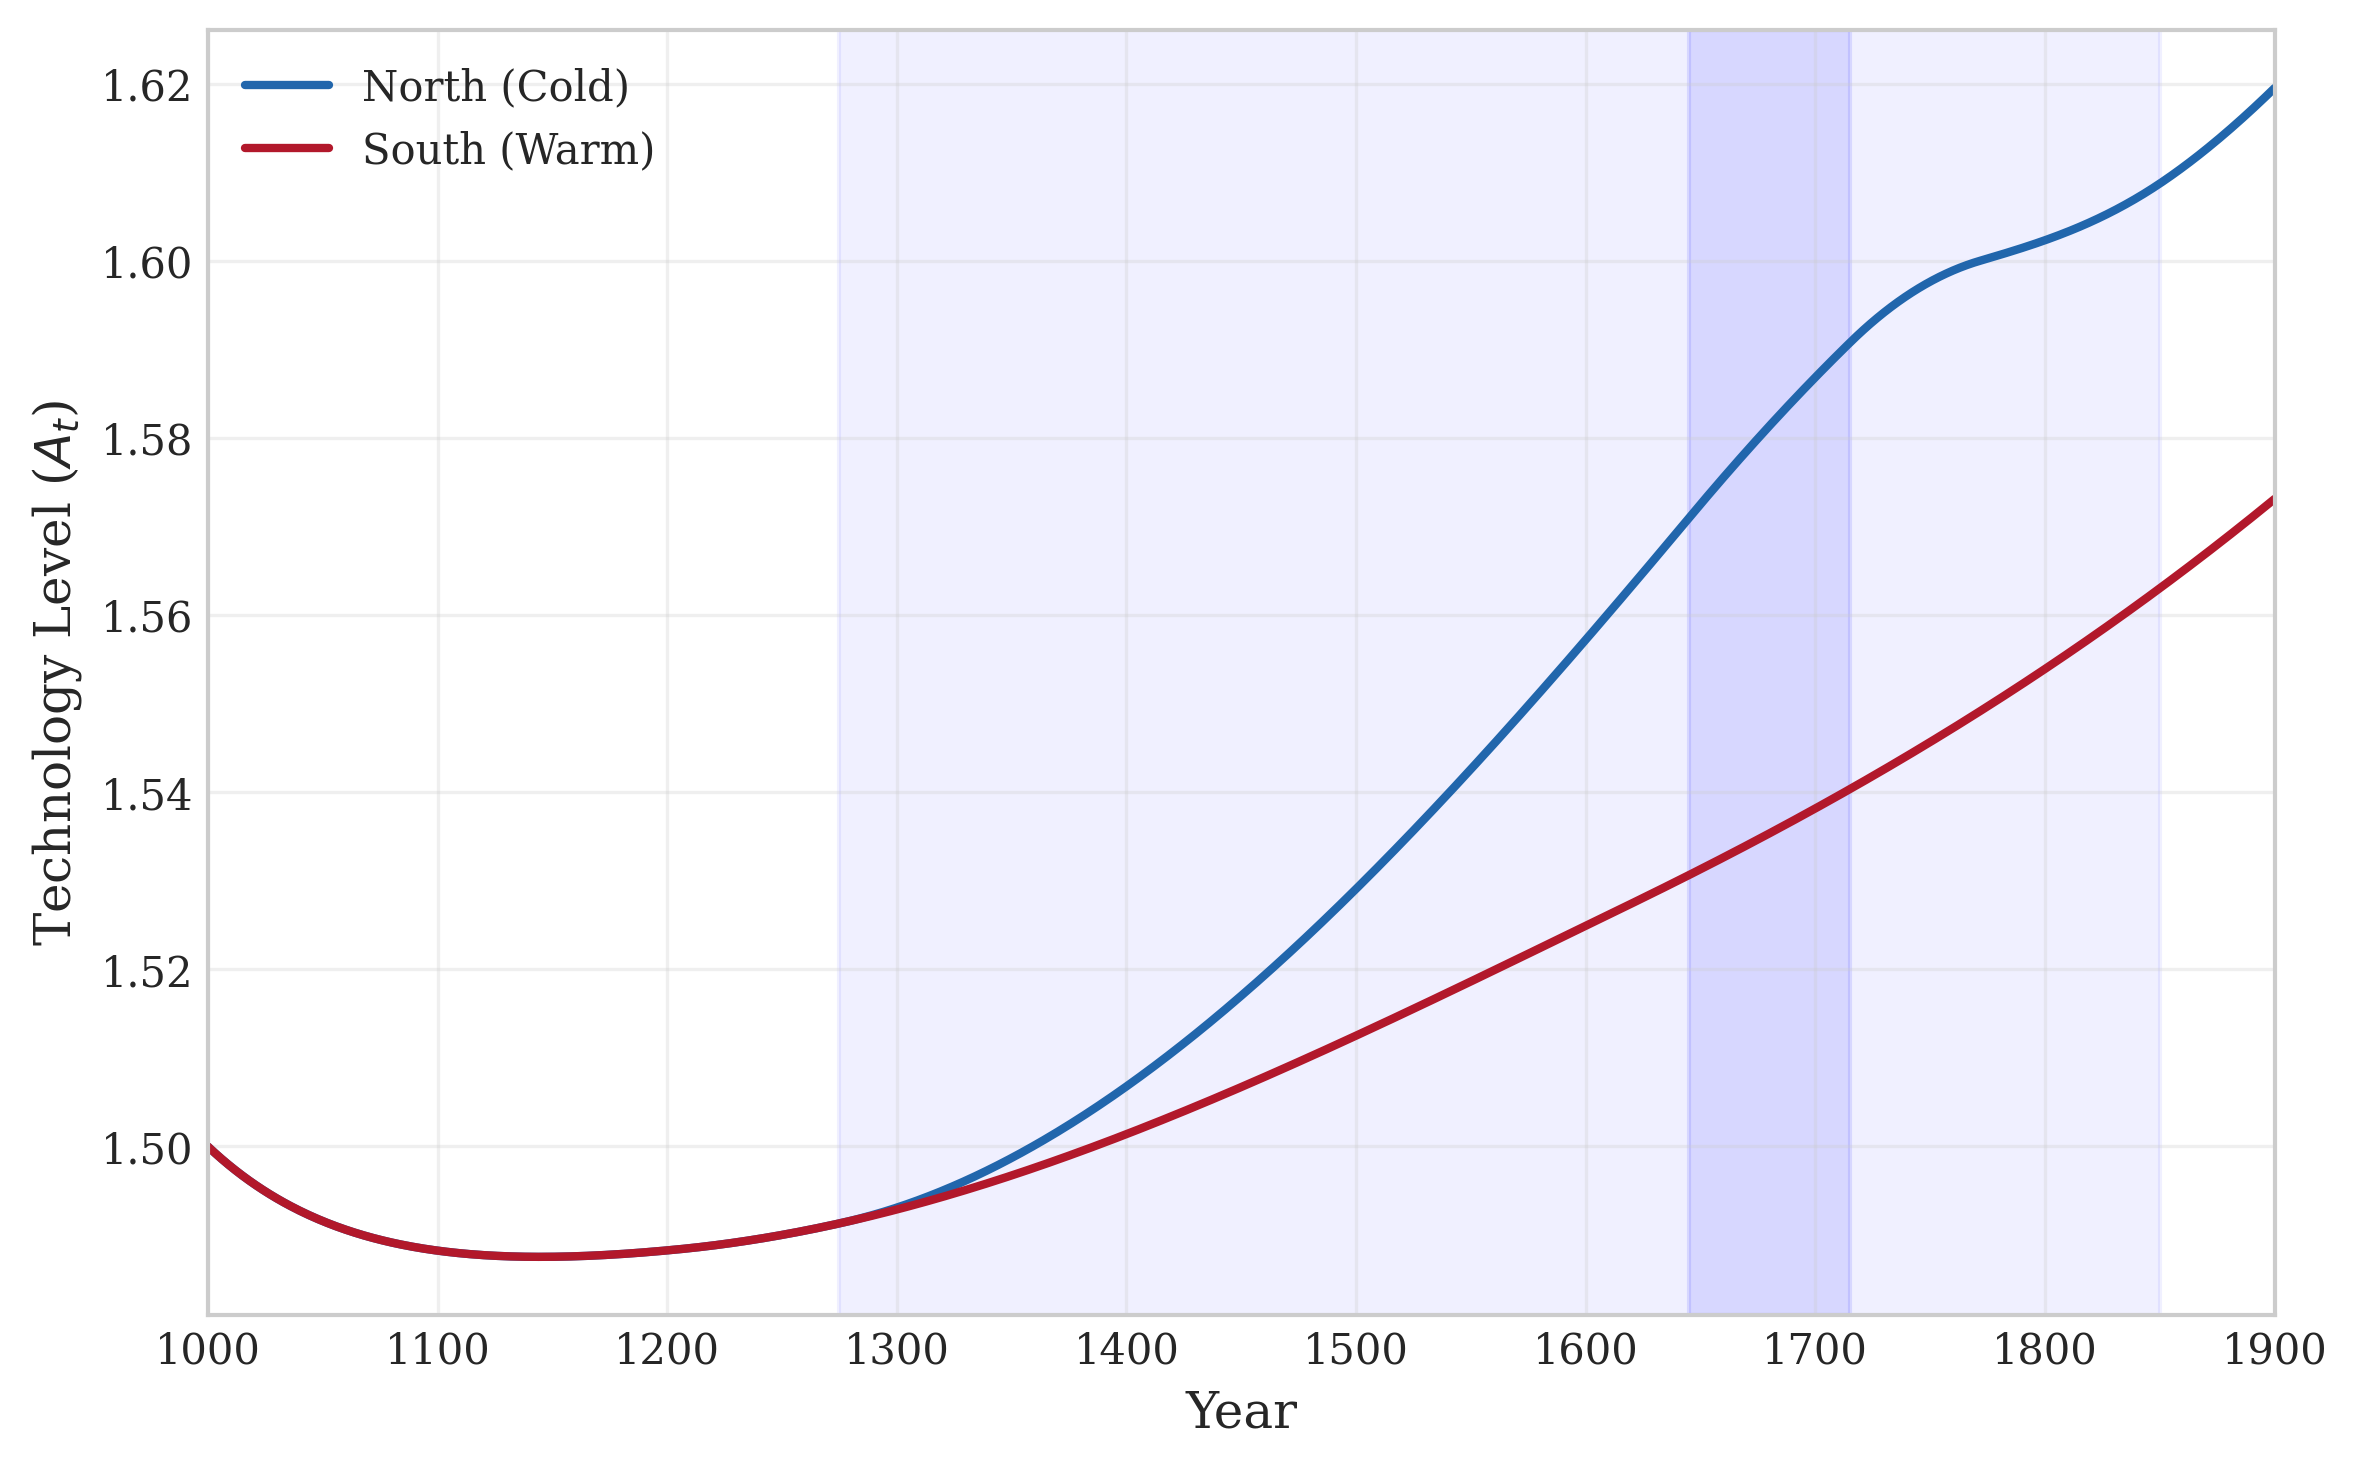
\includegraphics[width=0.9\textwidth]{../grafici_galor/gw_comparison_technology.png}
  \caption{\textbf{Technological Divergence.} The North (Cold) accumulates technology faster than the South (Warm) due to higher labor input during the Little Ice Age, generating a persistent productivity advantage.}
  \label{fig:sim_technology}
\end{figure}

\subsubsection*{Escape from the subsistence trap}

\Cref{fig:sim_consumption} presents per capita consumption. Both regions begin near subsistence (\(c \approx \bar{y} = 0.90\)). During the LIA, Northern consumption drops slightly as the climate shock reduces effective productivity, but the accumulated technology eventually lifts consumption above the Southern level. This is the mechanism of the ``escape'': the forced accumulation of knowledge, though painful in the short run, generates a long-run surplus. The North breaks away from the subsistence floor, while the South remains trapped.

\begin{figure}[h!]
  \centering
  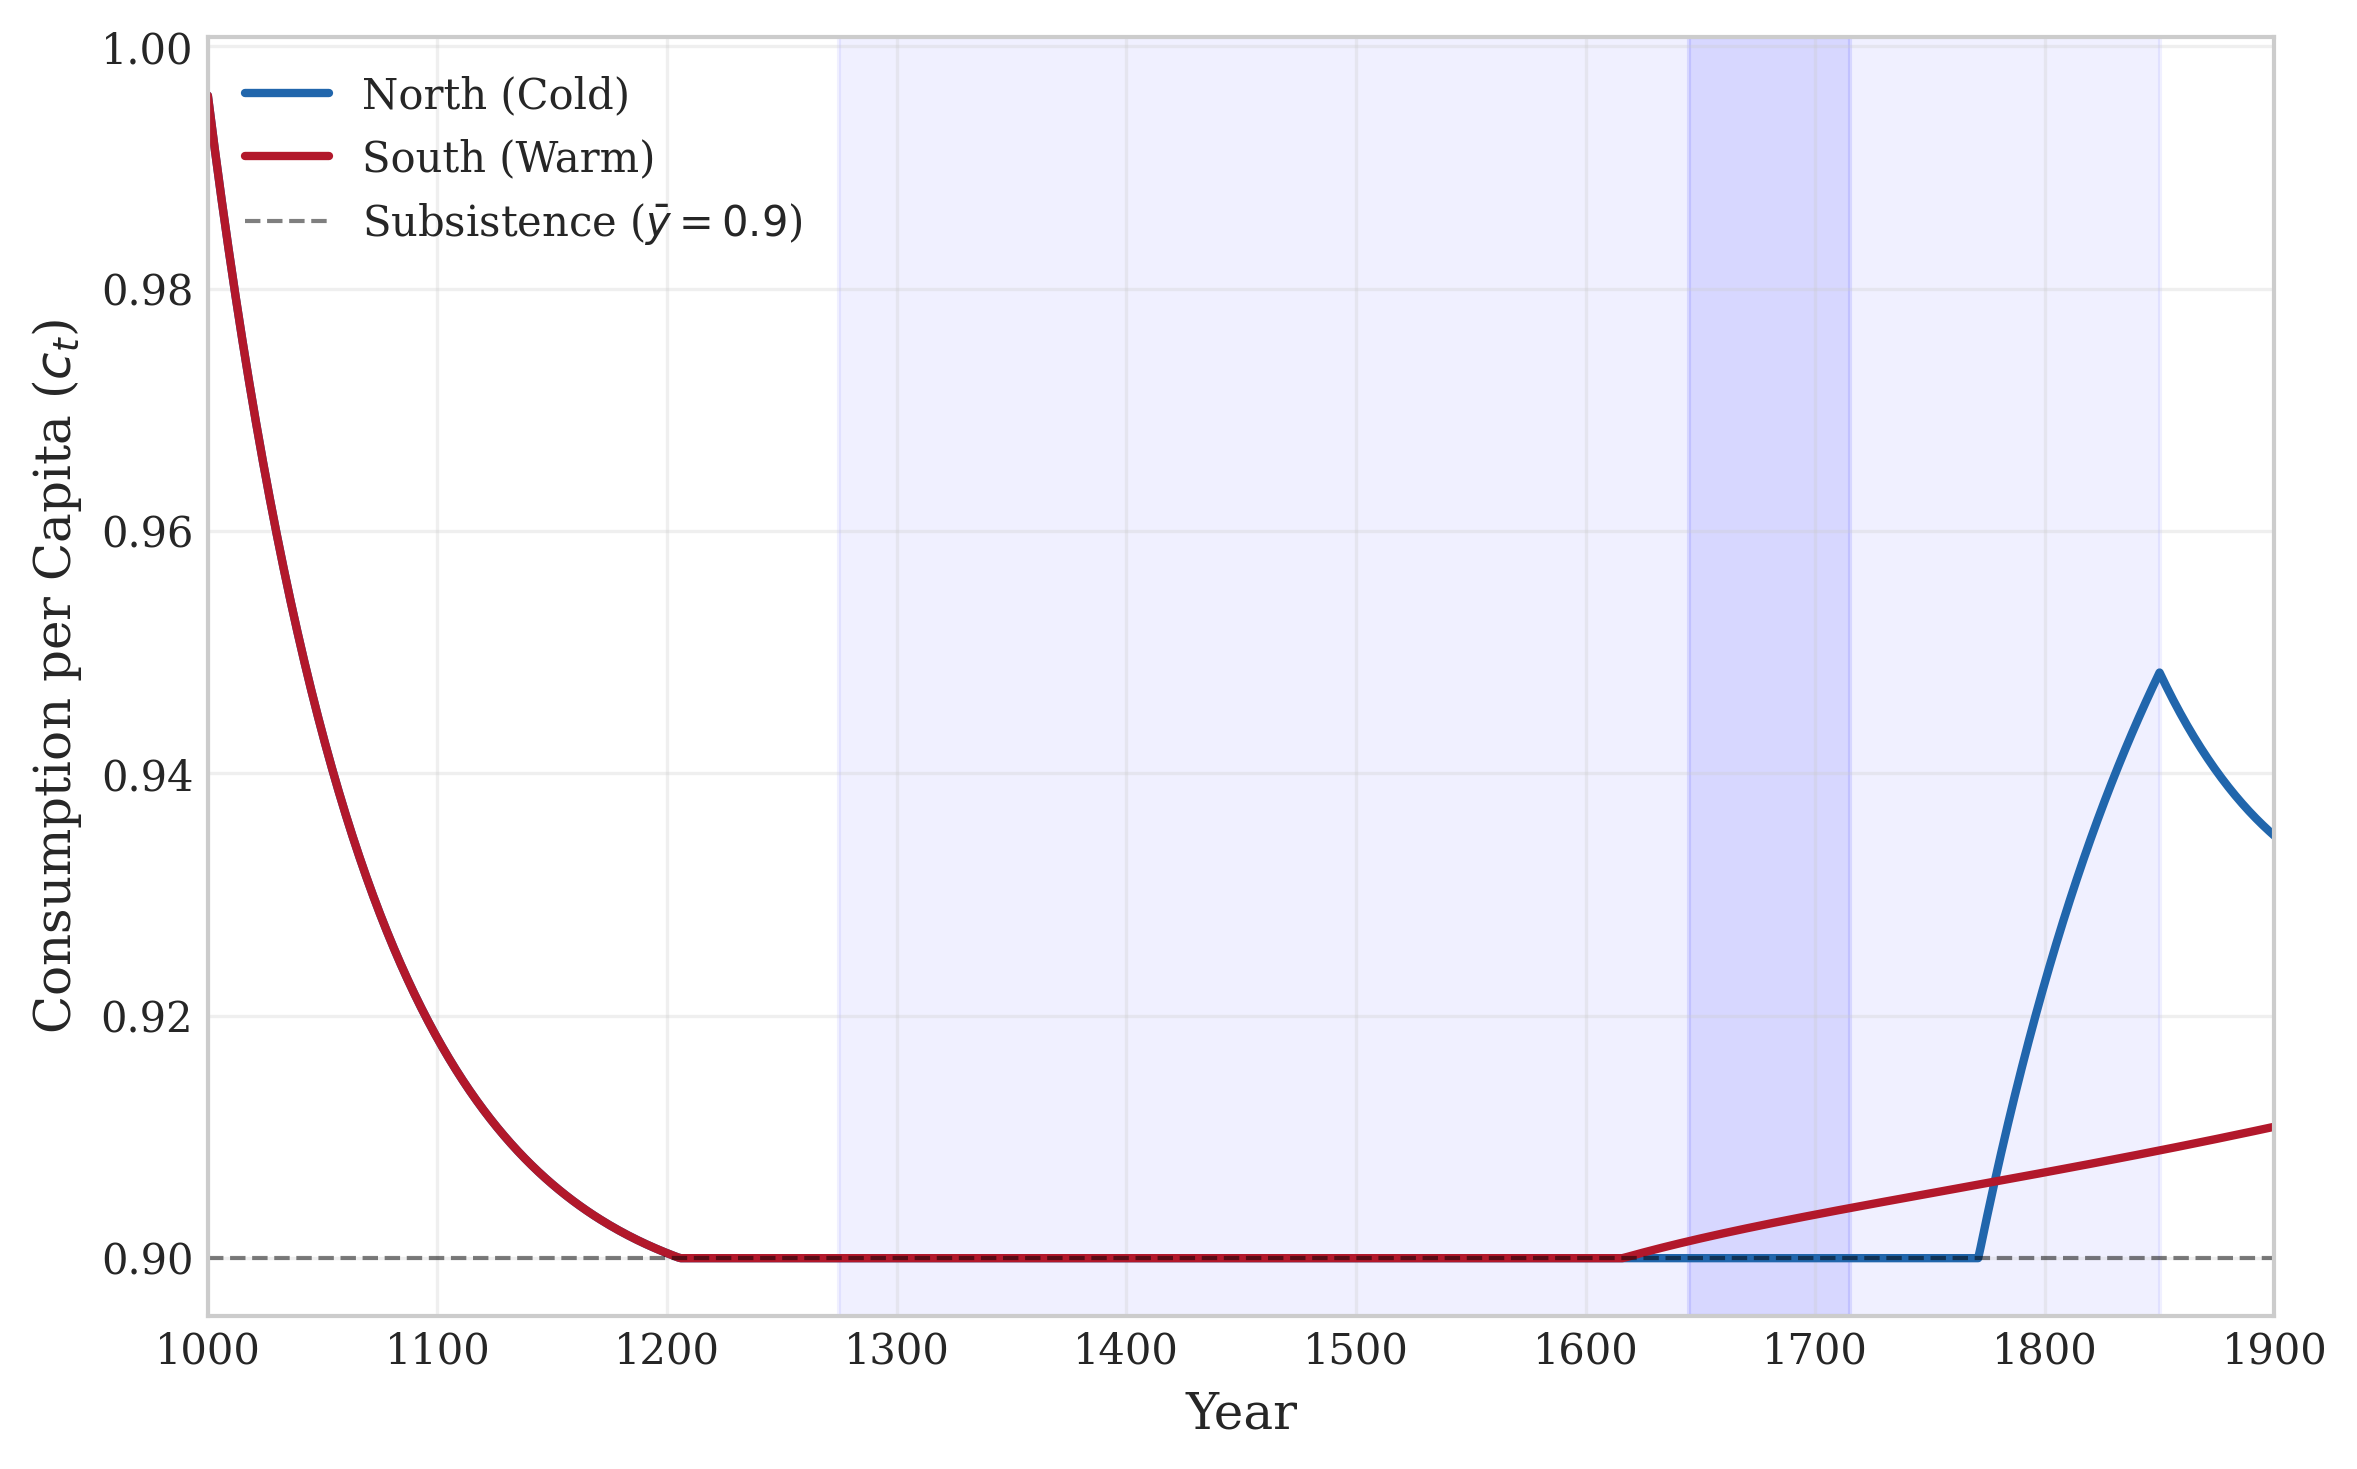
\includegraphics[width=0.9\textwidth]{../grafici_galor/gw_comparison_consumption.png}
  \caption{\textbf{Escape from the Trap.} Consumption per capita in the North (Cold) eventually exceeds the South (Warm). The dashed line marks the subsistence threshold \(\bar{y}\).}
  \label{fig:sim_consumption}
\end{figure}

\section{Limitations and Discussion}
Our model focuses on the closed-economy labor-leisure channel and abstracts from several factors. On trade: while the LIA likely spurred grain flows from South to North, our mechanism emphasizes local production responses and does not model inter-regional exchange. On institutions: we treat institutions as endogenous to technology, but the LIA likely interacted with pre-existing frameworks, such as the Enclosures, that are not explicitly modeled. On epidemics: we distinguish the LIA from the Black Death, but the interaction between climate, nutrition, and disease is complex and is simplified here into the survival rule.

\section{Conclusion}

This paper examines the climatic origins of the Agricultural Revolution and the Great Divergence using a subsistence labor--leisure model. The prolonged stress of the Little Ice Age, we argue, drove institutional and technological innovation in Northern Europe. Unlike previous models that treat technological progress as purely exogenous or density-dependent, our framework identifies environmental adversity as the primary trigger of the ``Industrious Revolution.''

Our simulations demonstrate that the North's early lead was not accidental. The necessity of maintaining subsistence in a colder climate forced households into a high-labor, high-innovation regime. This industriousness, combined with a technological lead that eventually triggered the demographic transition, allowed the North to escape the Malthusian trap while the South remained stagnant. Whether the same mechanism can explain within-country variation---between Scotland and England, or between Castile and Aragon---remains an open question.

\emergencystretch 3em
\printbibliography

\end{document}
